\documentclass[11pt]{article}

% ---- Packages ----
\usepackage[utf8]{inputenc}
\usepackage[T1]{fontenc}
\usepackage{amsmath,amssymb}
\usepackage{graphicx}
\usepackage{booktabs}
\usepackage{multirow}
\usepackage{hyperref}
\hypersetup{colorlinks=true,linkcolor=blue,citecolor=blue,urlcolor=blue}
\usepackage[margin=1in]{geometry}
\usepackage{xcolor}
\usepackage{caption}
\usepackage{subcaption}
\usepackage{enumitem}
\usepackage{natbib}
\bibliographystyle{unsrtnat}

% ---- Placeholder command for TODOs ----
\newcommand{\todo}[1]{\textcolor{red}{\textbf{[TODO: #1]}}}
\newcommand{\fillnum}[1]{\textcolor{blue}{\textbf{#1}}}

% ============================================================================
\title{ClusterNet: Disentangling When and Why Graph Neural Networks\\
Surpass Classical Community Detection on Biological Networks}

\author{
  R.~Sapna\textsuperscript{1},
  Harikeshav Karthik\textsuperscript{2},
  Karthik Raman\textsuperscript{1,3,4}
  \\[6pt]
  \textsuperscript{1}Bhupat and Jyoti Mehta School of Biosciences, Department of Biotechnology,\\
  Indian Institute of Technology (IIT) Madras, Chennai 600036, India\\
  \textsuperscript{2}School of Biomedical Engineering, IIT (BHU) Varanasi, India\\
  \textsuperscript{3}Wadhwani School of Data Science and AI, IIT Madras, Chennai 600036, India\\
  \textsuperscript{4}Centre for Integrative Biology and Systems mEdicine (IBSE), IIT Madras\\[6pt]
  Correspondence: \texttt{kraman@iitm.ac.in}
}
\date{}

\begin{document}
\maketitle

% ============================================================================
\begin{abstract}
We present ClusterNet, a unified benchmark evaluating 30 classical and 8 graph-neural-network (GNN) community detection algorithms across three tiers of increasing biological realism: synthetic LFR graphs, attributed social networks, and four human molecular networks (SIGNOR, GRN, BioGRID, GTEx). Our results establish a clear conditional: GNNs outperform classical methods only when informative node features are available and network topology alone leaves community boundaries ambiguous. Feature ablation confirms this quantitatively---GO annotations boost GNN modularity by 56--100\% on sparse regulatory networks but add negligible signal on the dense GTEx co-expression graph. Beyond partitioning accuracy, we demonstrate that GNNs provide biological interpretability inaccessible to classical methods: GAT attention weights preferentially attend to activating over inhibiting edges ($p = 3.2 \times 10^{-16}$) and correlate negatively with transcription-factor out-degree (Spearman $\rho = -0.92$, $p < 10^{-269}$), revealing learned sensitivity to regulatory specificity without explicit pathway supervision. Perturbation analysis further shows that contrastive GNNs (DGI, NMI\,=\,0.51) maintain partition stability under targeted TF knockout while supervised architectures collapse (NMI\,$<$\,0.14). We release ClusterNet as an open-source package with reproducible pipelines and practitioner guidelines for all 38 methods.
\end{abstract}

% ============================================================================
\section{Introduction}
\label{sec:introduction}

Networks pervade biology at every scale: protein interactions form complexes, gene regulatory circuits coordinate cellular programs, metabolic enzymes assemble into pathways, and neural populations organize into functional areas.
The communities within these networks often correspond to functional modules, from signaling cascades to co-regulated gene sets to protein complexes~\citep{santo_fortunato_d0b5bf4d, choobdar_dream_2019}.
Detecting these communities reliably is not merely an algorithmic exercise; it is a gateway to biological discovery, from identifying disease modules to predicting drug targets~\citep{gergely_palla_c9fbd5c7, albert__aszl__barab_si_ebeab141}.

The toolbox for this task has grown enormously.
Classical methods based on modularity optimization~\citep{vincent_d__blondel_eead1c1a, traag_leiden_2019}, information compression~\citep{martin_rosvall_68b9da5e}, spectral decomposition~\citep{ulrike_von_luxburg_b9cd91aa}, and Bayesian inference~\citep{peixoto_sbm_2014} operate on topology alone and remain the workhorses of biological network analysis.
Graph neural networks (GNNs) represent a fundamentally different paradigm: they jointly learn from network topology \emph{and} node attributes through message-passing, potentially uncovering communities that topology alone misses.
Architectures like GCN~\citep{thomas_kipf_d7121869}, GAT~\citep{velickovic_gat_2018}, VGAE~\citep{thomas_kipf_6638cd97}, and differentiable pooling methods~\citep{tsitsulin_dmon_2023, bianchi_mincut_2020} have shown promise on citation graph benchmarks.
Yet a fundamental question persists: \emph{do these methods genuinely improve community detection on biological networks, where success is measured not by label agreement but by whether detected modules correspond to real pathways, regulatory circuits, or disease mechanisms?}
And perhaps more importantly for the AI community: \emph{what can we learn from how GNNs solve this problem that we cannot learn from classical algorithms?}

Three gaps in the current literature have prevented clear answers.
First, no existing benchmark evaluates both classical and GNN methods under identical conditions on the same networks~\citep{andrea_lancichinetti_37f463ca, zhao_yang_133f261c, xing_su_d49e541e}.
Second, standard synthetic benchmarks (LFR)~\citep{andrea_lancichinetti_125b2a5e} lack node attributes entirely, making them unable to test the central promise of GNNs.
Third, biological evaluations typically use a single PPI network with fold-enrichment as the only metric~\citep{choobdar_dream_2019}, ignoring the diversity of network types now available (directed regulatory networks, signed signaling networks) and the richer metrics they demand.

We designed ClusterNet to address these gaps through a three-tier evaluation (Figure~\ref{fig:lfr_accuracy} illustrates Tier~1; full details in Methods):

\begin{enumerate}[leftmargin=*]
  \item \textbf{LFR synthetic networks} (Tier~1) establish a controlled baseline: these topology-only graphs with known communities allow us to measure what happens when GNNs have \emph{no} feature advantage. We demonstrate that they underperform here, confirming that their power must originate elsewhere.

  \item \textbf{Attributed social networks} (Tier~2) introduce real node features (Cora, CiteSeer, Amazon Photo) and a systematic ablation isolating the contribution of features versus topology. We demonstrate that the GNN advantage is directly proportional to feature informativeness and inversely proportional to graph density.

  \item \textbf{Biological networks} (Tier~3) provide the real test. Four human molecular networks (GTEx co-expression, a gene regulatory network, BioGRID PPI, and SIGNOR signaling) are evaluated by Gene Ontology and KEGG pathway enrichment, feed-forward loop preservation, sign coherence, perturbation robustness, and AI interpretability analyses. No ground-truth partition exists here; biological coherence is the only judge.
\end{enumerate}

\noindent This design traces a deliberate arc: from ``GNNs underperform without features'' (Tier~1) through ``features help on sparse attributed graphs'' (Tier~2) to ``what do GNNs uniquely reveal about biology?'' (Tier~3).

Our main contributions are:
\begin{itemize}[leftmargin=*]
  \item \textbf{ClusterNet}: the first head-to-head comparison of 30~classical and 8~GNN algorithms across all three tiers under identical protocols, released as an open-source Python package unifying CDLib, graph-tool, and PyTorch Geometric.
  \item A feature ablation on both social and biological networks that quantifies \emph{when} node attributes help GNN-based community detection, establishing that the GNN advantage is network-density-dependent and feature-quality-dependent.
  \item An AI interpretability analysis demonstrating that GNNs learn biologically meaningful structure without explicit supervision: GAT attention weights discriminate activating from inhibiting regulatory edges, concentrate on specific rather than promiscuous regulators, and embedding visualizations reveal pathway-aligned latent clusters.
  \item A multi-metric biological evaluation going beyond modularity: GO/KEGG enrichment, FFL preservation, sign coherence, disease module overlap, and a perturbation analysis showing that transcription-factor knockout disrupts community structure far more than random gene removal.
  \item Practical recommendations for biologists choosing among these 38 algorithms.
\end{itemize}


% ============================================================================
\section{Related Work}
\label{sec:related}

\paragraph{Classical algorithm benchmarks.}
The LFR benchmark~\citep{andrea_lancichinetti_125b2a5e} remains the standard synthetic testbed for community detection.
Lancichinetti and Fortunato~\citep{andrea_lancichinetti_37f463ca} compared a dozen algorithms on LFR, establishing mixing parameter sweeps as the primary evaluation methodology.
Yang et al.~\citep{zhao_yang_133f261c} extended this to 8 algorithms with additional network size analysis.
Dao et al.~\citep{vinh_loc_dao_5627549f} provided a broader comparative evaluation across 12 methods.
These studies are limited to classical algorithms and synthetic or small social networks, typically below 5{,}000 nodes.

\paragraph{GNN-based community detection.}
Several GNN architectures have been adapted for community detection, each with a different inductive bias.
DMoN~\citep{tsitsulin_dmon_2023} directly optimizes a differentiable modularity loss; MinCutPool~\citep{bianchi_mincut_2020} minimizes a relaxed normalized cut.
DGI~\citep{velickovic_dgi_2019} takes a representation-learning approach, maximizing mutual information between node and graph representations, followed by $k$-means on the learned embeddings.
VGAE~\citep{thomas_kipf_6638cd97} learns a latent space via variational inference on graph-structured data.
Su et al.~\citep{xing_su_d49e541e} survey these methods comprehensively but do not compare them against classical algorithms under identical experimental conditions.

\paragraph{Biological network module identification.}
The DREAM Challenge~\citep{choobdar_dream_2019} benchmarked module identification methods on six heterogeneous biological networks, establishing the importance of domain-specific evaluation.
However, it predated the current generation of GNN methods and did not evaluate GNNs.
Biological benchmarks typically rely on PPI networks from STRING with fold-enrichment as the sole quality measure, missing the diversity of directed, signed, and regulatory networks that are now available from resources such as SIGNOR~\citep{signor_2020} and BioGRID~\citep{biogrid_2023}.

\paragraph{Feature ablation and the role of node attributes.}
While node classification benchmarks routinely evaluate GNNs on attributed graphs~\citep{sen_cora_2008, shchur_amazon_2018}, the community detection literature lacks a systematic ablation isolating the contribution of features versus topology.
Our work fills this gap by running identical GNN architectures with real, structural, and random features on the same graphs.


% ============================================================================
\section{Methods}
\label{sec:methods}

\subsection{Algorithms}
\label{sec:algorithms}

We evaluate 38 community detection algorithms organized into two paradigms (Table~\ref{tab:algorithms}).

\paragraph{Classical algorithms (30).}
We include representative methods from seven families:
\emph{modularity-based} (Louvain~\citep{vincent_d__blondel_eead1c1a}, Leiden~\citep{traag_leiden_2019}, FastGreedy, Walktrap),
\emph{information-theoretic} (Infomap~\citep{martin_rosvall_68b9da5e}),
\emph{spectral} (spectral clustering~\citep{ulrike_von_luxburg_b9cd91aa}, leading eigenvector),
\emph{statistical inference} (SBM, Nested SBM~\citep{peixoto_sbm_2014}, Expectation--Maximization),
\emph{label propagation and local methods} (Label Propagation~\citep{santo_fortunato_93a74814}, Spinglass, SCAN, Async Fluid, Surprise),
\emph{resolution-based} (CPM, RB-Pots, RBer-Pots),
\emph{overlapping} (Angel, Demon, $k$-Clique~\citep{gergely_palla_c9fbd5c7}),
\emph{competition-winning} methods from the DREAM Challenge~\citep{choobdar_dream_2019} (SCORE, TeamCS, BigS2, CSBIO-IITM2),
and \emph{additional heuristics} (AGDL, DER, GDMP2, SimNet, SVT, Tusk).
All classical algorithms operate on topology alone and require no node features.

\paragraph{GNN-based algorithms (8).}
We evaluate four categories of neural methods, all implemented in PyTorch Geometric~\citep{fey_pyg_2019}:
\begin{itemize}[leftmargin=*,nosep]
  \item \emph{Unsupervised differentiable pooling}: DMoN~\citep{tsitsulin_dmon_2023} (modularity loss), MinCutPool~\citep{bianchi_mincut_2020} (normalized-cut loss).
  \item \emph{Self-supervised representation learning}: VGAE~\citep{thomas_kipf_6638cd97} + $k$-means, DGI~\citep{velickovic_dgi_2019} + $k$-means.
  \item \emph{Semi-supervised classification}: GCN~\citep{thomas_kipf_d7121869} and GAT~\citep{velickovic_gat_2018} trained on partial labels, with community assignment via argmax.
  \item \emph{Ablation baselines}: MLP + $k$-means (features only, no message passing), Node2Vec~\citep{grover_node2vec_2016} + $k$-means (topology only, no features).
\end{itemize}
All GNN methods use a two-layer encoder with hidden dimension 128, trained for 600 epochs with the Adam optimizer (learning rate $10^{-3}$).
For unsupervised and representation-learning methods, the number of clusters $K$ is set to the Louvain-derived value on each graph; for semi-supervised methods, $K$ equals the number of ground-truth classes (LFR, social) or GO Slim categories (biological).
Detailed mathematical formulations, objective functions, and computational complexity for all 38 algorithms are provided in the Supplementary Material (Section~1, Table~S0).

\begin{table}[t]
\centering
\caption{Summary of all 38 algorithms evaluated. \emph{Type} indicates the paradigm; \emph{Features} indicates whether the algorithm uses node attributes; \emph{Labels} indicates whether supervision is required.}
\label{tab:algorithms}
\small
\begin{tabular}{llccc}
\toprule
\textbf{Algorithm} & \textbf{Family} & \textbf{Type} & \textbf{Features} & \textbf{Labels} \\
\midrule
Louvain, Leiden, FastGreedy, Walktrap & Modularity & Classical & No & No \\
Infomap & Information-theoretic & Classical & No & No \\
Spectral, Leading Eigenvector & Spectral & Classical & No & No \\
SBM, Nested SBM, EM & Statistical inference & Classical & No & No \\
Label Prop., Spinglass, SCAN & Local/propagation & Classical & No & No \\
CPM, RB-Pots, RBer-Pots & Resolution & Classical & No & No \\
Async Fluid, Surprise & Density/surprise & Classical & No & No \\
Angel, Demon, $k$-Clique & Overlapping & Classical & No & No \\
SCORE, TeamCS, BigS2, CSBIO-IITM2 & DREAM-derived & Classical & No & No \\
AGDL, DER, GDMP2, SimNet, SVT, Tusk & Other heuristics & Classical & No & No \\
\midrule
DMoN, MinCutPool & Diff. pooling & GNN & Yes & No \\
VGAE+$k$M, DGI+$k$M & Representation & GNN & Yes & No \\
GCN, GAT & Semi-supervised & GNN & Yes & Yes \\
MLP+$k$M & Feature baseline & GNN & Yes & No \\
Node2Vec+$k$M & Topology baseline & GNN & No$^*$ & No \\
\bottomrule
\end{tabular}

\vspace{2pt}
{\footnotesize $^*$Node2Vec learns embeddings from random walks on topology; node features are ignored.}
\end{table}


\subsection{Datasets}
\label{sec:datasets}

\subsubsection{Tier~1: LFR Synthetic Networks}

We use the Lancichinetti--Fortunato--Radicchi (LFR) benchmark~\citep{andrea_lancichinetti_125b2a5e} in three configurations:

\begin{itemize}[leftmargin=*,nosep]
  \item \textbf{Accuracy benchmark:} $N=1{,}000$ nodes, $\mu \in [0.10, 0.80]$ in steps of 0.02 (36~values), 3 realizations per $\mu$, average degree $\bar{k}=15$, degree exponent $\gamma=2$, community size range $[20, 50]$.
  \item \textbf{Scalability benchmark:} $N \in \{500,\; 1{,}000,\; 2{,}500,\; 5{,}000,\; 25{,}000\}$, $\mu=0.15$, 3 realizations per size.
  \item \textbf{Hierarchical benchmark:} $N=1{,}000$, $(\mu_1, \mu_2)$ grid with $\mu_1, \mu_2 \in \{0.1, 0.2, 0.3\}$ (9~configurations), macro-community sizes $[100, 300]$, micro-community sizes $[10, 50]$, 3 realizations per pair.
\end{itemize}
For hierarchical experiments, Nested SBM inference uses graph-tool's full MCMC procedure to recover nested partitions at both micro and macro scales.

For GNN methods on LFR networks, node features consist of structural properties: degree, clustering coefficient, PageRank, and Laplacian eigenvector positional encodings (16 dimensions total).
For semi-supervised GCN/GAT, ground-truth community labels with 20\% training fraction are provided, with ablation at 40\%, 60\%, and 80\% label fractions.

\subsubsection{Tier~2: Attributed Social Networks}

We use three standard attributed graph benchmarks (Table~\ref{tab:social_datasets}), each providing real-valued node features and ground-truth class labels:

\begin{table}[h]
\centering
\caption{Social network dataset statistics.}
\label{tab:social_datasets}
\small
\begin{tabular}{lrrrrr}
\toprule
\textbf{Dataset} & \textbf{Nodes} & \textbf{Edges} & \textbf{Classes} & \textbf{Features} & \textbf{Homophily} \\
\midrule
Cora~\citep{sen_cora_2008} & 2{,}708 & 5{,}278 & 7 & 1{,}433 & 0.81 \\
CiteSeer~\citep{sen_cora_2008} & 3{,}327 & 4{,}552 & 6 & 3{,}703 & 0.736 \\
Amazon Photo~\citep{shchur_amazon_2018} & 7{,}650 & 119{,}081 & 8 & 745 & 0.827 \\
\bottomrule
\end{tabular}
\end{table}

For the feature ablation experiment, each GNN is run with three feature settings:
(i)~\textbf{Real features}: original node attributes (bag-of-words for citation networks, product features for Amazon Photo);
(ii)~\textbf{Structural features}: 16-dimensional vectors comprising degree, clustering coefficient, PageRank, and spectral embedding;
(iii)~\textbf{Random features}: i.i.d.\ Gaussian noise matching the dimensionality of real features.
This ablation isolates the contribution of informative attributes versus architectural capacity.
For classical statistical blockmodels (\texttt{sbm}, \texttt{nested\_sbm}), graph-tool estimation frequently failed on these attributed graphs; reported implementations fell back to Louvain-style modularity optimization, yielding partitions duplicate of other modularity methods.
We therefore exclude \texttt{sbm}, \texttt{nested\_sbm}, and \texttt{nested\_sbm\_coarse} from social-tier rankings and narrative summaries.

\subsubsection{Tier~3: Biological Networks}

We assemble four human molecular networks spanning distinct interaction types (Table~\ref{tab:bio_datasets}).
This portfolio deliberately covers the major data modalities in computational biology: undirected co-expression (GTEx), directed regulation (GRN), undirected physical interactions (BioGRID PPI), and directed signed signaling (SIGNOR).
PPI networks are a natural benchmarking choice because protein complexes and functional modules provide well-characterized community-like structures~\citep{choobdar_dream_2019}; the additional network types test robustness beyond this standard setting.

\begin{table}[h]
\centering
\caption{Biological network dataset statistics.}
\label{tab:bio_datasets}
\small
\begin{tabular}{llrrlll}
\toprule
\textbf{Network} & \textbf{Type} & \textbf{Nodes} & \textbf{Edges} & \textbf{Directed} & \textbf{Signed} & \textbf{Features} \\
\midrule
GTEx~\citep{gtex_2020} & Co-expression & 5{,}694 & 1{,}423{,}975 & No & No & TPM (PCA-128) \\
Human GRN & Regulatory & 17{,}348 & 264{,}393 & Yes & No & TPM (PCA-128) \\
BioGRID~\citep{biogrid_2023} & PPI & 15{,}876 & 865{,}950 & No & No & GO binary (3{,}886) \\
SIGNOR~\citep{signor_2020} & Signaling & 5{,}815 & 17{,}052 & Yes & Yes & GO + sign-degree (2{,}382) \\
\bottomrule
\end{tabular}
\end{table}

GTEx co-expression edges are derived from Pearson correlation $\geq 0.9$ across 55{,}000 tissue samples from the GTEx v8 TPM matrix~\citep{gtex_2020}.
The Human GRN captures transcription-factor--target relationships with directed, weighted edges.
Node features for expression-based networks (GTEx, GRN) are 128-dimensional PCA projections of TPM expression profiles; for interaction-based networks (BioGRID, SIGNOR), features are binary Gene Ontology term vectors augmented with sign-aware degree features for SIGNOR.
Directed edges are symmetrized for community detection while raw directionality is retained for feed-forward loop (FFL) enumeration and sign coherence analysis.


\subsection{Evaluation Metrics}
\label{sec:metrics}

\paragraph{Partition quality (Tiers 1--2).}
Where ground-truth communities are available, we use Adjusted Mutual Information (AMI)~\citep{vinh_ami_2010} as the primary metric.
AMI corrects for chance agreement (unlike raw NMI, which is biased toward partitions with many small communities) and returns 0 for random partitions regardless of $K$.
We additionally report NMI for comparability with prior work and modularity~\citep{m__e__j__newman_cfc12888} as a secondary unsupervised measure, though we note that modularity suffers from a well-documented resolution limit~\citep{santo_fortunato_d0b5bf4d}: it cannot resolve communities smaller than $\sqrt{2m}$ edges and systematically favors coarse partitions.
We therefore never use modularity as the sole criterion for comparing algorithms; it is reported alongside AMI and biological metrics to illustrate this very tension.
We also report the number of detected communities $K$ and wall-clock runtime.

\paragraph{Biological relevance (Tier 3).}
In the absence of ground-truth partitions, we evaluate biological coherence through four complementary metrics:
\begin{itemize}[leftmargin=*,nosep]
  \item \textbf{GO/KEGG enrichment}: For each community with $\geq 5$ genes, we query g:Profiler~\citep{gprofiler_2019} for significant Gene Ontology (Biological Process, Molecular Function, Cellular Component) and KEGG pathway enrichments ($p \leq 0.05$, Benjamini--Hochberg correction). We report the fraction of tested communities with at least one significant term.
  \item \textbf{FFL preservation} (GRN only): The fraction of enumerated feed-forward loops~\citep{shen_orr_ffl_2002, milo_motifs_2002} whose three nodes reside in the same community.
  \item \textbf{Sign coherence} (SIGNOR only): The fraction of intra-community edges sharing the dominant sign (activation or inhibition), averaging over communities with $\geq 2$ internal edges.
  \item \textbf{Modularity}: Newman--Girvan modularity computed on the undirected, absolute-weight graph.
\end{itemize}

\paragraph{Perturbation robustness (GRN only).}
To assess structural sensitivity to biologically meaningful perturbations, we apply four perturbation tests to the Human GRN and measure partition stability (NMI, AMI between perturbed and baseline partitions), modularity change, and FFL preservation change:
\begin{enumerate}[leftmargin=*,nosep]
  \item \textbf{TF knockout}: removal of the top-5 and top-10 transcription factors by out-degree.
  \item \textbf{Edge dropout}: random removal of 5\%, 10\%, 20\%, and 30\% of edges.
  \item \textbf{Hub gene removal}: removal of the top 1\%, 2\%, and 5\% of genes by degree.
  \item \textbf{Random gene removal} (control): removal of 5 and 10 randomly selected genes.
\end{enumerate}


\subsection{Experimental Setup}
\label{sec:setup}

All experiments ran on a single NVIDIA RTX 5090 GPU instance (Vast.ai), with 32~GB VRAM and 64~GB system RAM under Ubuntu 22.04.
Classical algorithms ran on CPU; GNNs used GPU acceleration via PyTorch 2.10 and PyTorch Geometric 2.4 (CUDA 13.0).
The full software environment comprises Python~3.10, igraph~0.11, graph-tool~2.59, cdlib~0.4, leidenalg~0.10, infomap~2.7, NetworkX~3.2, NumPy~1.26, SciPy~1.11, and scikit-learn~1.3; exact version pins are recorded in the repository.
Each GNN experiment was repeated over 3 random seeds; we report means.
Classical algorithms are deterministic (single run per network) except for stochastic methods, which were also run with 3 seeds.
A timeout of 600 seconds was enforced per algorithm per network; algorithms exceeding this threshold on a given network were pruned from subsequent larger networks (adaptive pruning).
All code is implemented in Python 3.10 and released as the ClusterNet package at \url{https://github.com/RamanLab/ClusterNet}.

\paragraph{GPU acceleration of classical algorithms.}
Among the 30 classical algorithms, two (SimNet and BigS2) support optional GPU acceleration via CuPy for their computationally intensive matrix denoising and spectral decomposition steps.
In our benchmarks, all classical algorithms were run on CPU to ensure a fair timing comparison across methods; GPU-accelerated variants are available in the released package.
More broadly, the majority of classical community detection algorithms are inherently sequential and graph-traversal-based (greedy modularity moves, random walks, label propagation, MCMC sampling), making them difficult to vectorize on SIMD architectures.
Spectral methods and matrix-factorization-based approaches (Spectral Clustering, SimNet, BigS2, SVT) are the most amenable to GPU porting via batched linear algebra (cuBLAS/cuSOLVER); Louvain and Leiden have recent RAPIDS cuGraph implementations but require fundamentally different parallel strategies (hash-based aggregation) that alter convergence guarantees.
We restrict our GPU benchmarks to the GNN paradigm, where tensor-parallel computation is native to the architecture, and note GPU-classical comparison as a direction for future work.


% ============================================================================
\section{Results}
\label{sec:results}

\subsection{Tier 1: LFR Synthetic Benchmarks}
\label{sec:results_lfr}

We begin with LFR synthetic graphs to establish a controlled baseline.
These networks have known communities defined purely by edge density, with no meaningful node attributes.
They answer a prerequisite question: how do GNNs perform when they cannot rely on features?

\subsubsection{Accuracy versus Mixing Parameter}

Complete numerical results (AMI at seven key $\mu$ values for all 38 algorithms) appear in Supplementary Table~S1; here we summarize the main patterns.
For visual clarity, figures in this section display a curated subset of algorithms representative of each paradigm family (top-ranked methods plus illustrative failure cases); full per-algorithm data are reported in the supplementary tables.

\begin{figure*}[t]
\centering
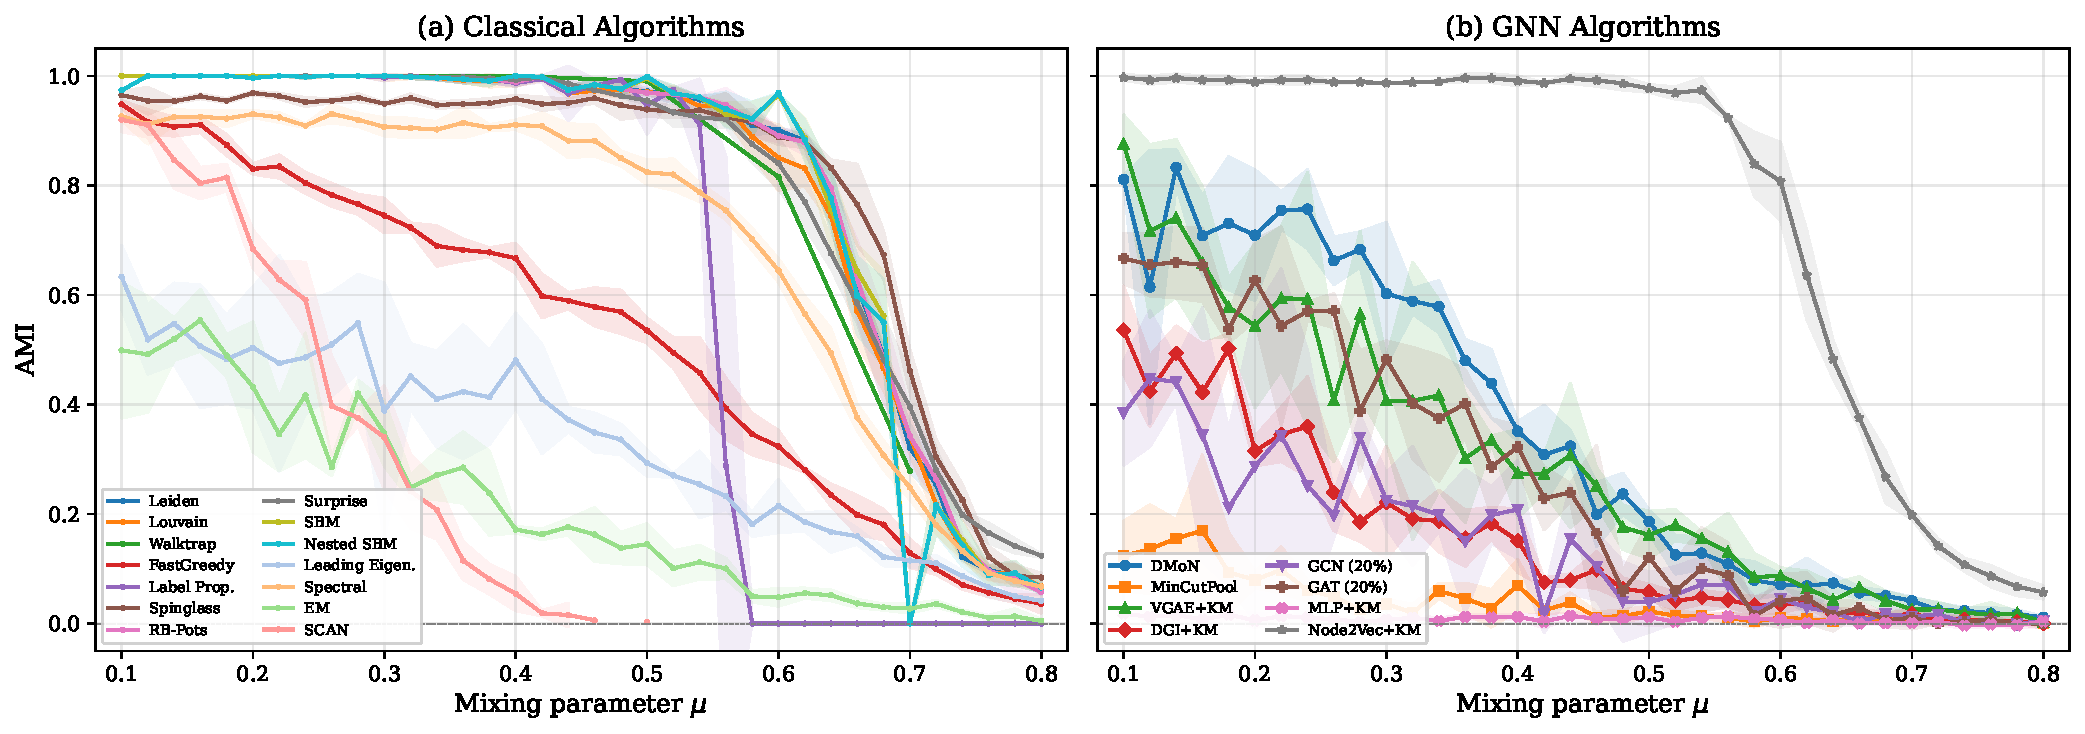
\includegraphics[width=\textwidth]{figures/fig1_lfr_accuracy.pdf}
\caption{AMI versus mixing parameter $\mu$ on the LFR accuracy benchmark ($N{=}1{,}000$). (a)~Classical algorithms with 95\% confidence bands across 3 realizations. (b)~GNN algorithms using only structural features (degree, clustering coefficient, PageRank, spectral PE). Node2Vec+KM, which learns embeddings from topology alone via random walks, substantially outperforms all message-passing GNNs.}
\label{fig:lfr_accuracy}
\end{figure*}

We find that when communities are well-separated ($\mu \leq 0.3$), most classical algorithms recover them perfectly.
Walktrap, Leiden, Louvain, CSBIO-IITM2, RB-Pots, and Nested SBM all reach AMI~$\approx 1.0$ in this regime (full results in Supplementary Table~S1).
The interesting differences emerge at higher mixing.
At $\mu = 0.5$, where community boundaries become genuinely ambiguous, TeamCS (AMI${}=1.00$), CSBIO-IITM2 ($0.997$), and Walktrap ($0.990$) still hold, while Label Propagation and Spectral have already degraded substantially.
By $\mu = 0.7$, even the best methods struggle: Spinglass ($0.462$) and Surprise ($0.396$) lead, while mainstream modularity methods collapse toward chance.

\textbf{GNNs without informative features are computationally expensive topology methods.}
On these attribute-free networks, every message-passing GNN falls well short of classical algorithms (Figure~\ref{fig:lfr_accuracy}b).
The exception is Node2Vec+KM (AMI${}=0.997$ at $\mu = 0.1$), but this is revealing: Node2Vec ignores node features entirely and learns from random walks, so it succeeds precisely because it sidesteps the uninformative structural features that handicap other GNNs.
Among GNNs that do consume features, VGAE+KM ($0.876$) and DMoN ($0.811$) lead at low mixing but remain far below the classical ceiling.
At $\mu = 0.5$ the gap is stark: Node2Vec+KM still manages $0.977$ while DMoN drops to $0.186$.
Semi-supervised GCN and GAT fare worst of all (peak AMI $< 0.67$ even at $\mu = 0.1$), confirming that degree and clustering coefficient do not carry sufficient community signal for message passing to exploit.

This result is important for what follows.
It establishes that GNNs are not inherently superior at community detection; their advantage, if any, must derive from informative node features. Tiers~2 and~3 test this prediction directly.

\begin{figure*}[t]
\centering
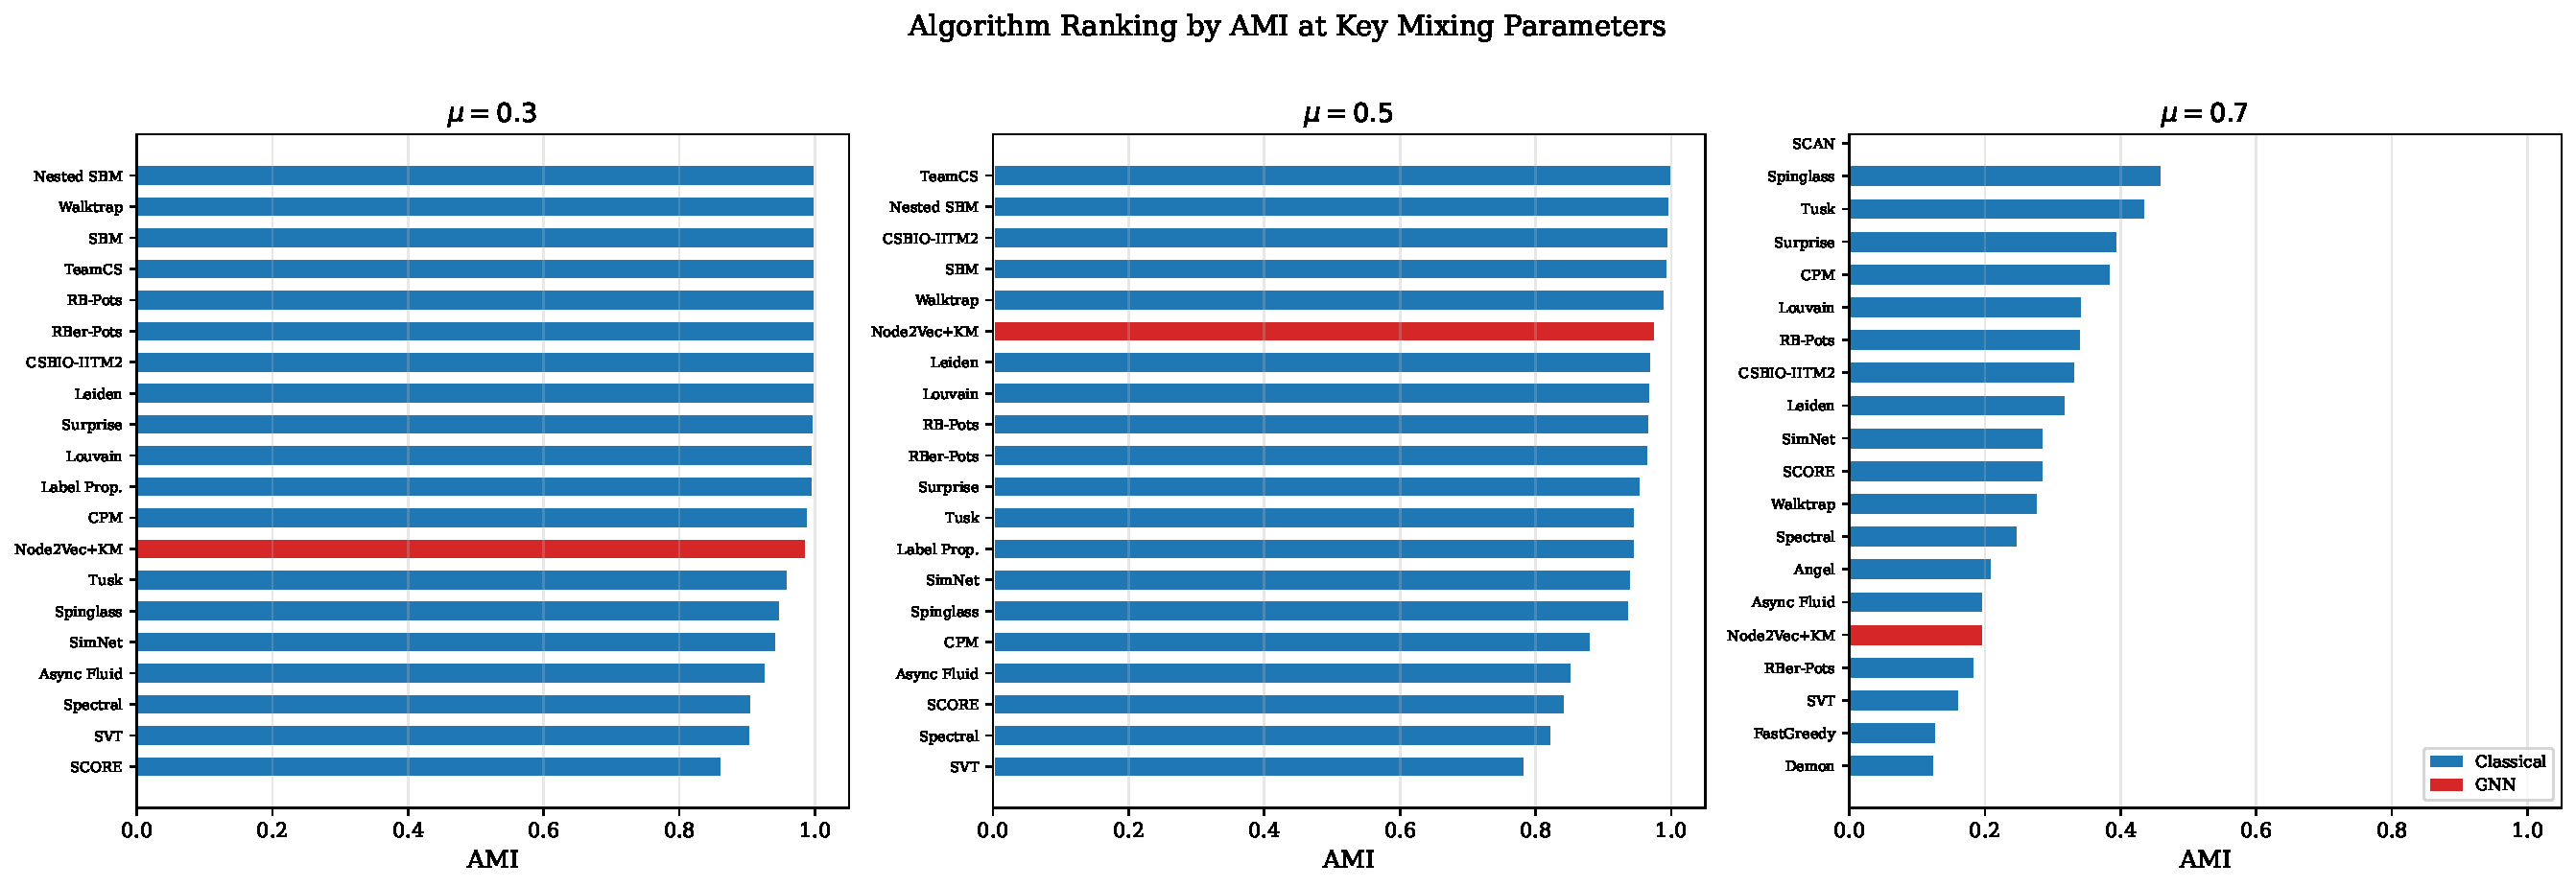
\includegraphics[width=\textwidth]{figures/fig5_lfr_ranking.pdf}
\caption{Top-20 algorithms ranked by mean AMI at three mixing parameters. Blue: classical; red: GNN. At $\mu = 0.3$ and $\mu = 0.5$, only Node2Vec+KM (a topology-only method) enters the top-20 among GNNs. At $\mu = 0.7$, no GNN exceeds the classical baseline.}
\label{fig:lfr_ranking}
\end{figure*}

The cross-paradigm ranking (Figure~\ref{fig:lfr_ranking}) makes the gap vivid.
At $\mu = 0.3$, Node2Vec+KM is the only GNN in the top 20, succeeding precisely because it ignores features.
At $\mu = 0.5$, it ranks fourth overall, above Leiden and Louvain, while no other GNN enters the top 15.
At $\mu = 0.7$, algorithms built for extreme mixing (SCAN, Spinglass, Surprise) dominate; GNNs are absent entirely.

\textbf{How algorithms fail.}
Examining the ratio $K_{\text{detected}} / K_{\text{true}}$ (Figure~\ref{fig:lfr_cluster_count}) reveals two distinct failure modes.
Some algorithms \emph{fragment}: Surprise at high $\mu$ reports 5$\times$ too many communities, splitting real clusters into pieces.
Others \emph{collapse}: Label Propagation and FastGreedy merge communities, detecting fewer than a third of the true number at $\mu \geq 0.6$.
Among GNNs, MinCutPool's cluster count is erratic, while DMoN and Node2Vec+KM stay closer to the true value (though this does not save their AMI scores).

\begin{figure*}[t]
\centering
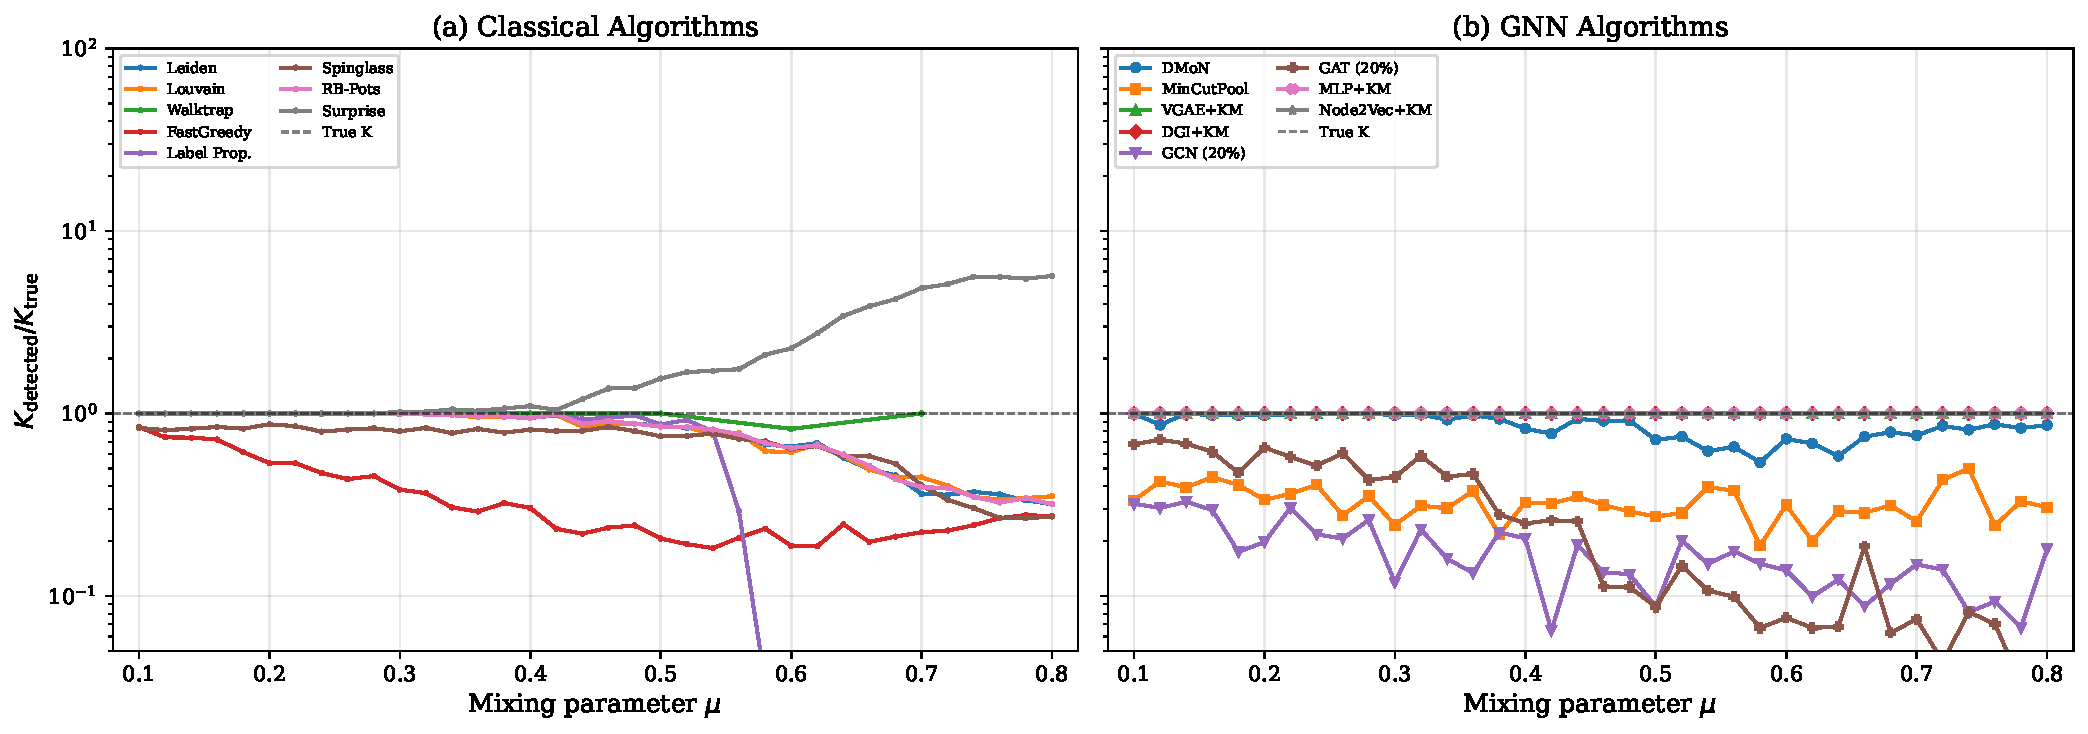
\includegraphics[width=\textwidth]{figures/fig6_lfr_cluster_count.pdf}
\caption{Detected-to-true community ratio $K_{\text{detected}} / K_{\text{true}}$ versus $\mu$ for selected classical (a) and GNN (b) algorithms, revealing fragmentation ($>1$) and collapse ($<1$) failure modes.}
\label{fig:lfr_cluster_count}
\end{figure*}

\subsubsection{Scalability}

Full scalability data (AMI and runtime at each $N$) is in Supplementary Table~S2.

\begin{figure*}[t]
\centering
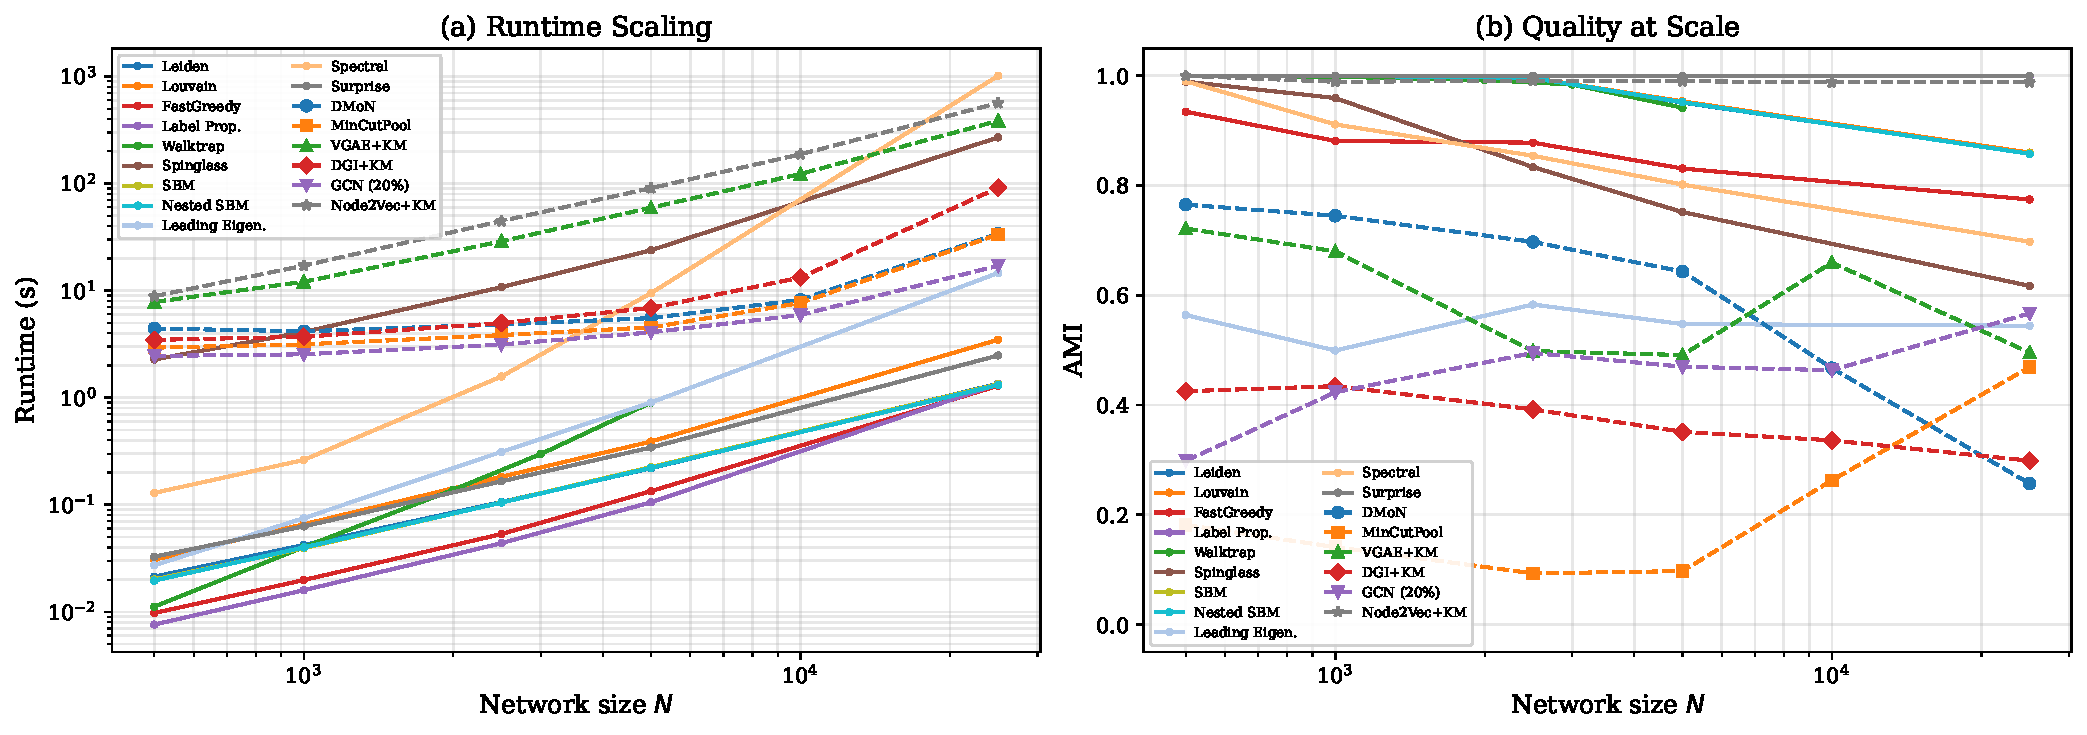
\includegraphics[width=\textwidth]{figures/fig2_lfr_scalability.pdf}
\caption{Runtime scaling (a) and partition quality at scale (b) from $N{=}500$ to $N{=}25{,}000$ ($\mu{=}0.15$). Solid lines: classical algorithms; dashed: GNNs. Louvain and Leiden maintain near-linear scaling with AMI${}\approx 1.0$ throughout. Node2Vec+KM preserves high AMI but becomes prohibitively slow at scale.}
\label{fig:lfr_scalability}
\end{figure*}

How do these methods scale? Figure~\ref{fig:lfr_scalability} and Supplementary Table~S2 track runtime and accuracy from 500 to 25{,}000 nodes at fixed $\mu = 0.15$.
The classical landscape separates cleanly by complexity class.
Label Propagation, Louvain, and Leiden finish the 25K-node graph in 1--3 seconds with perfect AMI; these remain the practical workhorses for large networks.
Spinglass and Spectral scale super-linearly and become impractical beyond a few thousand nodes.

GNNs incur a substantial runtime premium for no accuracy gain on these featureless graphs.
The fastest, GCN, takes 17s at 25K nodes; Node2Vec+KM requires over 9 minutes.
Moreover, most GNNs degrade in quality as the graph grows: DMoN drops to AMI${}=0.257$ and DGI+KM to $0.299$ at $N{=}25{,}000$, while Leiden maintains perfect recovery at a fraction of the cost.
Node2Vec+KM remains the exception (AMI${}=0.988$ at scale), reinforcing that its topology-only approach avoids the pitfalls of message-passing on uninformative features.

\subsubsection{Hierarchical Community Detection}

\begin{figure*}[t]
\centering
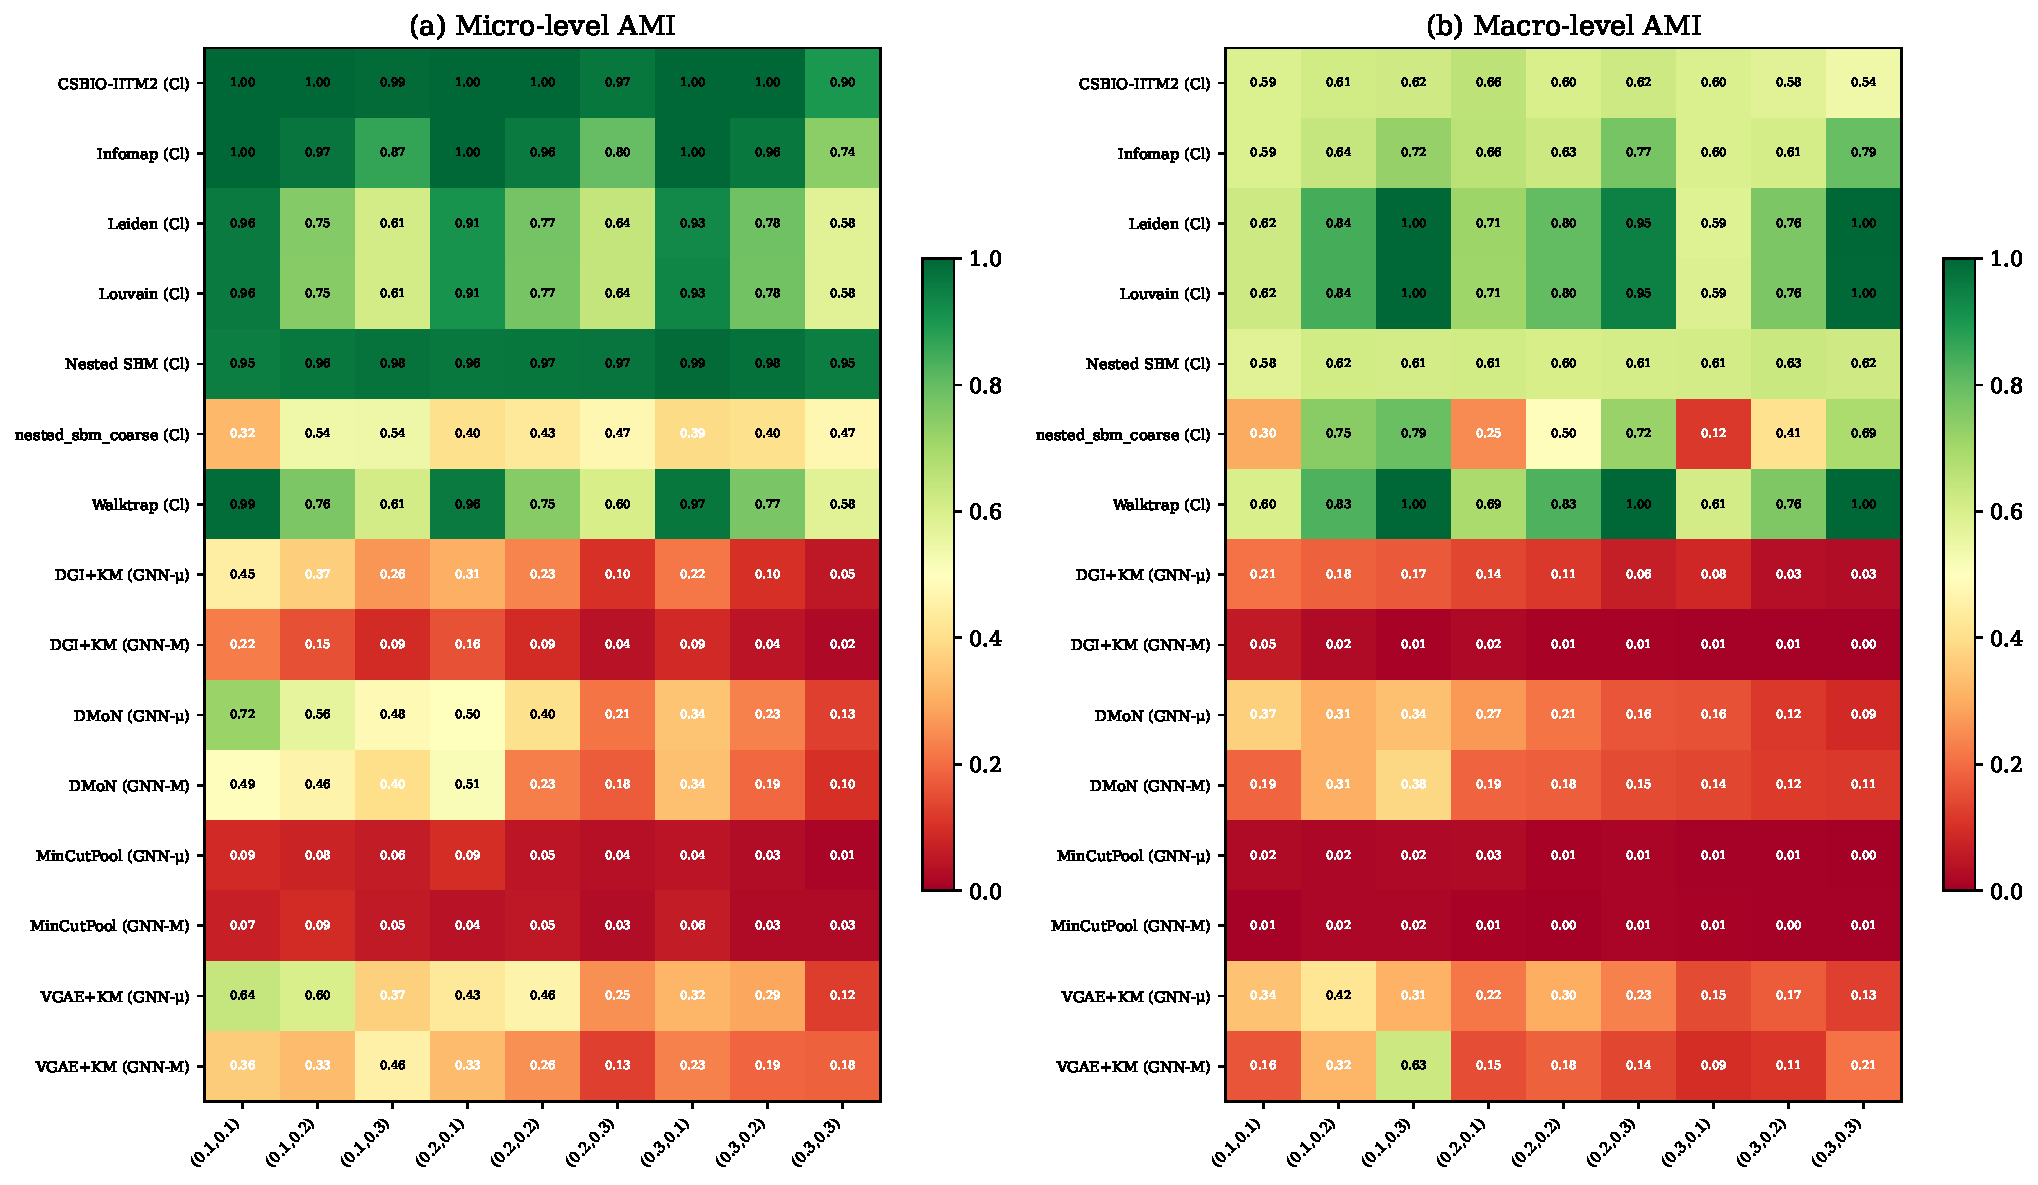
\includegraphics[width=\textwidth]{figures/fig3_lfr_hierarchical.pdf}
\caption{Micro-level (a) and macro-level (b) AMI on the LFR hierarchical benchmark across $(\mu_1, \mu_2) \in \{0.1, 0.2, 0.3\}^2$. Rows group classical (Cl) and GNN algorithms by micro ($\mu$) vs.\ macro (M) targets. Easy settings: CSBIO-IITM2 and Infomap reach perfect micro-AMI. At $(0.3,0.3)$, Leiden shifts to macro recovery (macro AMI${}\approx 1.0$, micro${}\approx 0.58$). Nested SBM at $(0.3,0.3)$ retains high micro AMI (${\approx}0.95$) with macro AMI near ${\approx}0.62$, i.e.\ a different trade-off than Leiden.}
\label{fig:lfr_hierarchical}
\end{figure*}

Real biological networks contain nested structure: metabolic pathways nest within broader functional modules, which nest within cellular compartments.
The hierarchical benchmark (Figure~\ref{fig:lfr_hierarchical}) tests whether algorithms can resolve both scales simultaneously.

A revealing trade-off emerges among classical methods.
At the easiest setting $(0.1, 0.1)$, most algorithms recover fine-grained (micro) communities well: CSBIO-IITM2 and Infomap achieve perfect micro-AMI with moderate macro recovery ($0.59$).
However, at $(0.3, 0.3)$, where both scales are harder to distinguish, different algorithms make fundamentally different trade-offs.
Leiden locks onto macro structure (macro-AMI${\approx}1.0$, micro-AMI${\approx}0.58$): its modularity objective merges small communities into large ones.
Nested SBM takes the opposite trade-off: it preserves micro-AMI at ${\approx}0.95$ while sacrificing macro recovery (${\approx}0.62$), using its Bayesian prior to resist the resolution limit.
Infomap offers the best compromise, retaining both micro ($0.739$) and macro ($0.795$) signal.

GNNs struggle here across the board.
Even the best (DMoN targeting micro-communities) reaches only $0.72$ at the easiest setting, well below classical methods.
MinCutPool essentially fails (micro $< 0.1$).
The pattern is consistent: without informative node features, GNNs have no advantage over algorithms designed specifically for topology.

\subsubsection{Supervised Label Fraction Ablation}

\begin{figure*}[t]
\centering
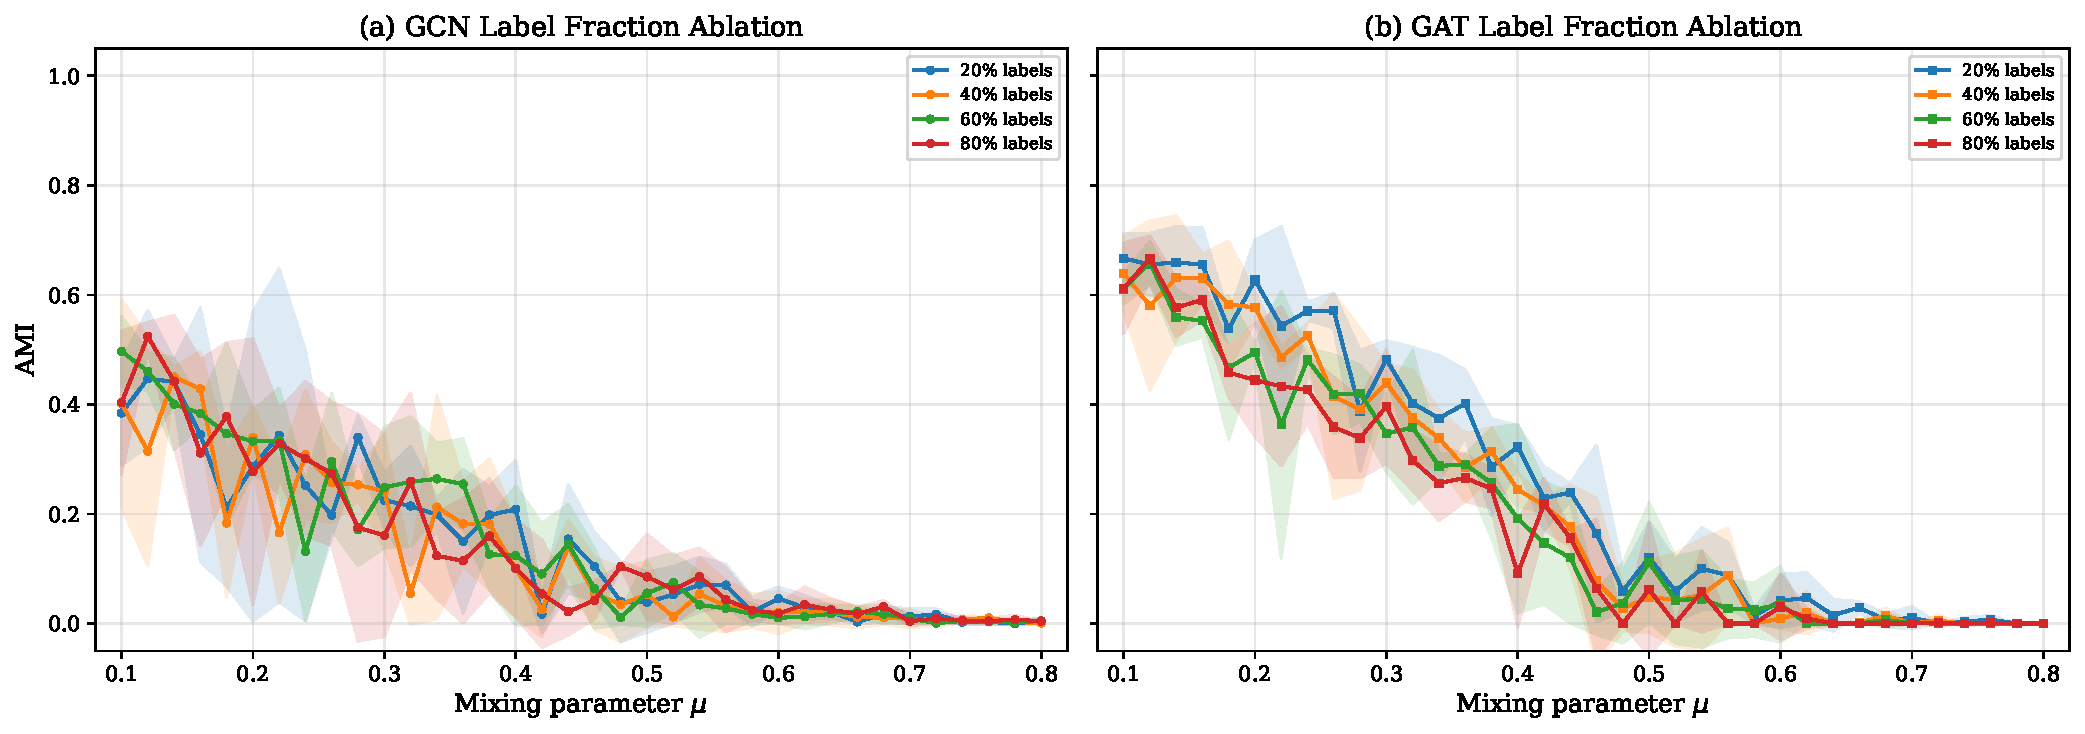
\includegraphics[width=\textwidth]{figures/fig4_lfr_label_ablation.pdf}
\caption{Label fraction ablation for semi-supervised GCN (a) and GAT (b) on LFR with structural features. Increasing label availability from 20\% to 80\% provides only marginal gains; both methods remain far below classical baselines at all $\mu$ values.}
\label{fig:lfr_label_ablation}
\end{figure*}

One might hypothesize that semi-supervised GNNs simply require more labels to succeed on LFR.
They do not.
Figure~\ref{fig:lfr_label_ablation} shows that increasing the training fraction from 20\% to 80\% produces no meaningful improvement, and occasionally degrades performance.
GAT at $\mu = 0.3$ gives AMI of $0.482$ (20\%), $0.439$ (40\%), $0.347$ (60\%), and $0.397$ (80\%): a non-monotonic trajectory that rules out label scarcity as the bottleneck.
The bottleneck is feature quality.
The same GCN and GAT architectures with informative bag-of-words features on social networks (Section~\ref{sec:results_social}) achieve far higher AMI, confirming that the LFR failure is not an architectural limitation but a data one.


\subsection{Tier 2: Attributed Social Networks}
\label{sec:results_social}

Having established that GNNs need informative features to justify their cost, we now ask: how much do features actually contribute, and when does topology suffice?
Social networks with ground-truth labels let us answer this via controlled ablation.

\subsubsection{Community Detection Sweep}

Full classical AMI values appear in Supplementary Table~S3 and the GNN ablation grid in Table~S4.
As in Tier~1, figures display the top-performing algorithms from each family for visual conciseness; complete rankings for all 38 methods are in the supplementary tables.

\begin{figure*}[t]
\centering
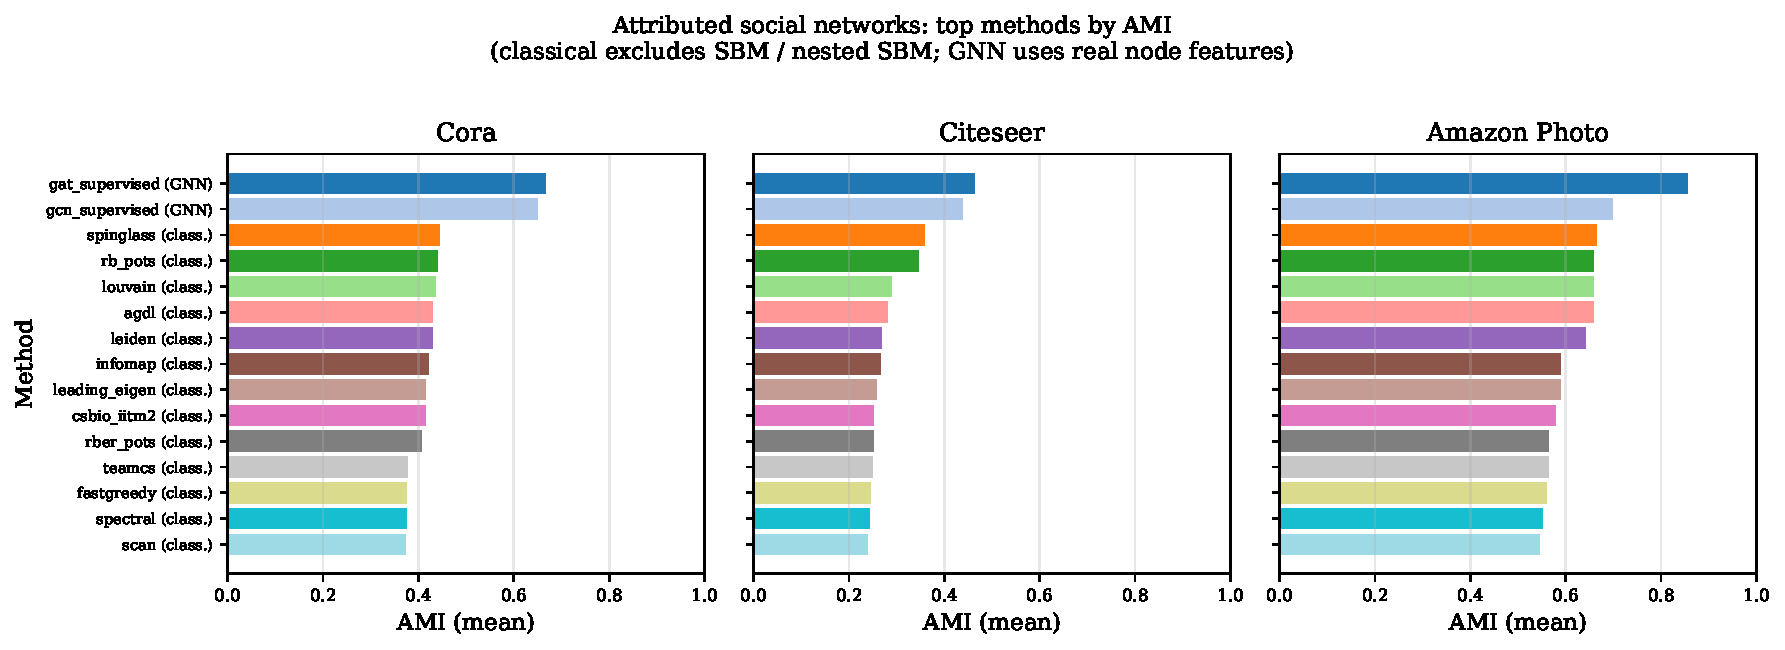
\includegraphics[width=\textwidth]{figures/fig_social_top_ami.pdf}
\caption{Top methods by mean AMI on Cora, CiteSeer, and Amazon Photo (15 per panel). GNN scores use \emph{real} node features (3 seeds). Semi-supervised GAT/GCN lead on all three graphs; classical modularity methods remain strongest among topology-only baselines.}
\label{fig:social_top_ami}
\end{figure*}

\begin{table}[t]
\centering
\caption{Top five methods per network by mean AMI (classical + GNN with real features). Full top-10 listings are in Supplementary Table~S5.}
\label{tab:social_top5}
\small
\begin{tabular}{llrr}
\toprule
\textbf{Network} & \textbf{Method} & \textbf{Type} & \textbf{AMI} \\
\midrule
Cora & \texttt{gat\_supervised} & GNN (real) & 0.667 \\
 & \texttt{gcn\_supervised} & GNN (real) & 0.650 \\
 & \texttt{fastgreedy} & classical & 0.445 \\
 & \texttt{spectral} & classical & 0.440 \\
 & \texttt{rber\_pots} & classical & 0.437 \\
\addlinespace[4pt]
Citeseer & \texttt{gat\_supervised} & GNN (real) & 0.464 \\
 & \texttt{gcn\_supervised} & GNN (real) & 0.439 \\
 & \texttt{spectral} & classical & 0.359 \\
 & \texttt{demon} & classical & 0.347 \\
 & \texttt{kclique} & classical & 0.288 \\
\addlinespace[4pt]
Amazon Photo & \texttt{gat\_supervised} & GNN (real) & 0.855 \\
 & \texttt{gcn\_supervised} & GNN (real) & 0.698 \\
 & \texttt{spinglass} & classical & 0.665 \\
 & \texttt{rb\_pots} & classical & 0.659 \\
 & \texttt{louvain} & classical & 0.658 \\
\addlinespace[4pt]
\bottomrule
\end{tabular}
\normalsize
\end{table}

The social networks reverse the LFR finding entirely.
With real bag-of-words features, GAT and GCN dominate: they top the AMI rankings on all three graphs (Table~\ref{tab:social_top5}, Figure~\ref{fig:social_top_ami}), reaching ${\approx}0.86$ (GAT) and $0.70$ (GCN) on Amazon Photo, well ahead of the best classical methods (Spinglass at ${\approx}0.67$, Louvain at ${\approx}0.59$).
Unsupervised GNNs (VGAE+KM, Node2Vec+KM) occupy the middle ground, tracking the stronger classical methods but falling short of semi-supervised performance.
The contrast with Tier~1 is unambiguous: these networks possess \emph{informative} features, and GNNs exploit them effectively.

\subsubsection{Feature Ablation}

\begin{figure*}[t]
\centering
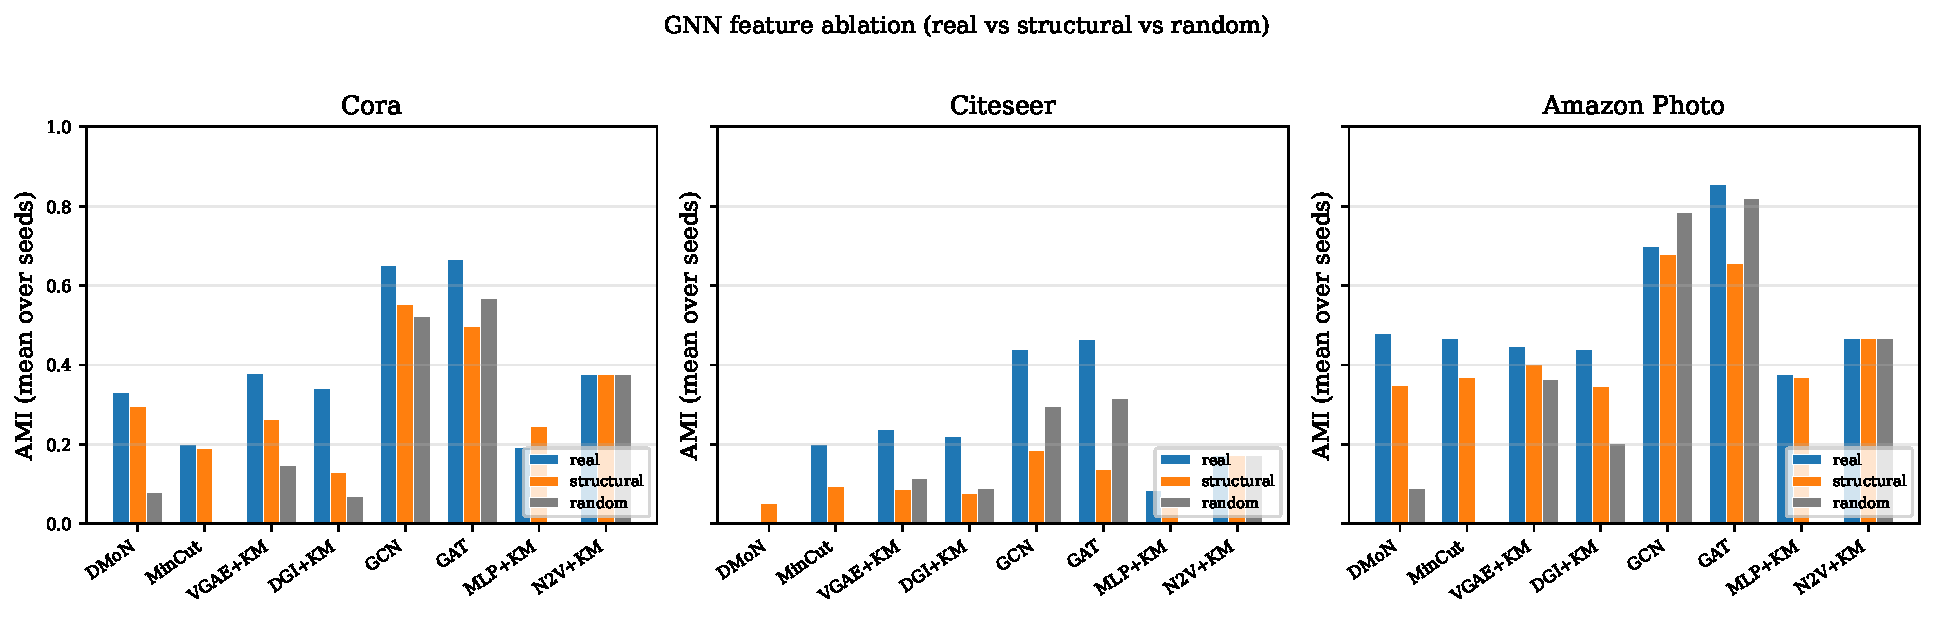
\includegraphics[width=\textwidth]{figures/fig_social_feature_ablation.pdf}
\caption{Mean AMI across three random seeds for each GNN architecture under real, structural-only, and random node features. Node2Vec+KM is invariant by construction. On Cora and CiteSeer, semi-supervised methods show large drops under random features; on Amazon Photo, GCN/GAT retain high AMI even with random attributes, indicating that supervision and dense topology dominate there.}
\label{fig:social_feature_ablation}
\end{figure*}

The ablation (Figure~\ref{fig:social_feature_ablation}; Supplementary Table~S4) pins down exactly where features matter.
On Cora and CiteSeer (sparse citation graphs), replacing real features with random noise drops GAT AMI from ${\approx}0.67$ to ${\approx}0.57$.
That gap quantifies the feature contribution: tangible but not dominant, and classical Leiden still competes without any features at all.
On Amazon Photo the picture changes: GAT with \emph{random} features still reaches AMI${\approx}0.82$, barely below the ${\approx}0.86$ with real attributes.
Here the dense topology and semi-supervised objective perform most of the work; product embeddings add only marginal signal.

Structural features (degree, clustering coefficient, spectral PE) land consistently between real and random, confirming they carry partial community information.
Node2Vec+KM, as expected, gives identical AMI regardless of feature setting because it never looks at node attributes.

The conclusion from Tier~2 is a principle we carry directly into the biological analysis: feature informativeness determines whether GNNs justify their computational cost.
On sparse graphs with meaningful attributes, the answer is affirmative.
On dense graphs where topology alone is rich, the answer is less definitive.
We now test whether this principle generalizes to real molecular networks.


\subsection{Tier 3: Biological Networks}
\label{sec:results_bio}

We now turn to the central question of this work: what happens when we move from labeled benchmarks to real biological networks where no ground truth exists and success must be judged by biological coherence?
We evaluate all 38 algorithms on four human molecular networks spanning distinct interaction types, using GO/KEGG enrichment, regulatory motif preservation, sign coherence, perturbation robustness, feature ablation, and AI interpretability analyses.
Full enrichment results are in Supplementary Table~S6, perturbation stability in Table~S7, and biological feature ablation in Table~S9.

\subsubsection{GO/KEGG Enrichment Analysis}

\begin{figure}[ht]
\centering
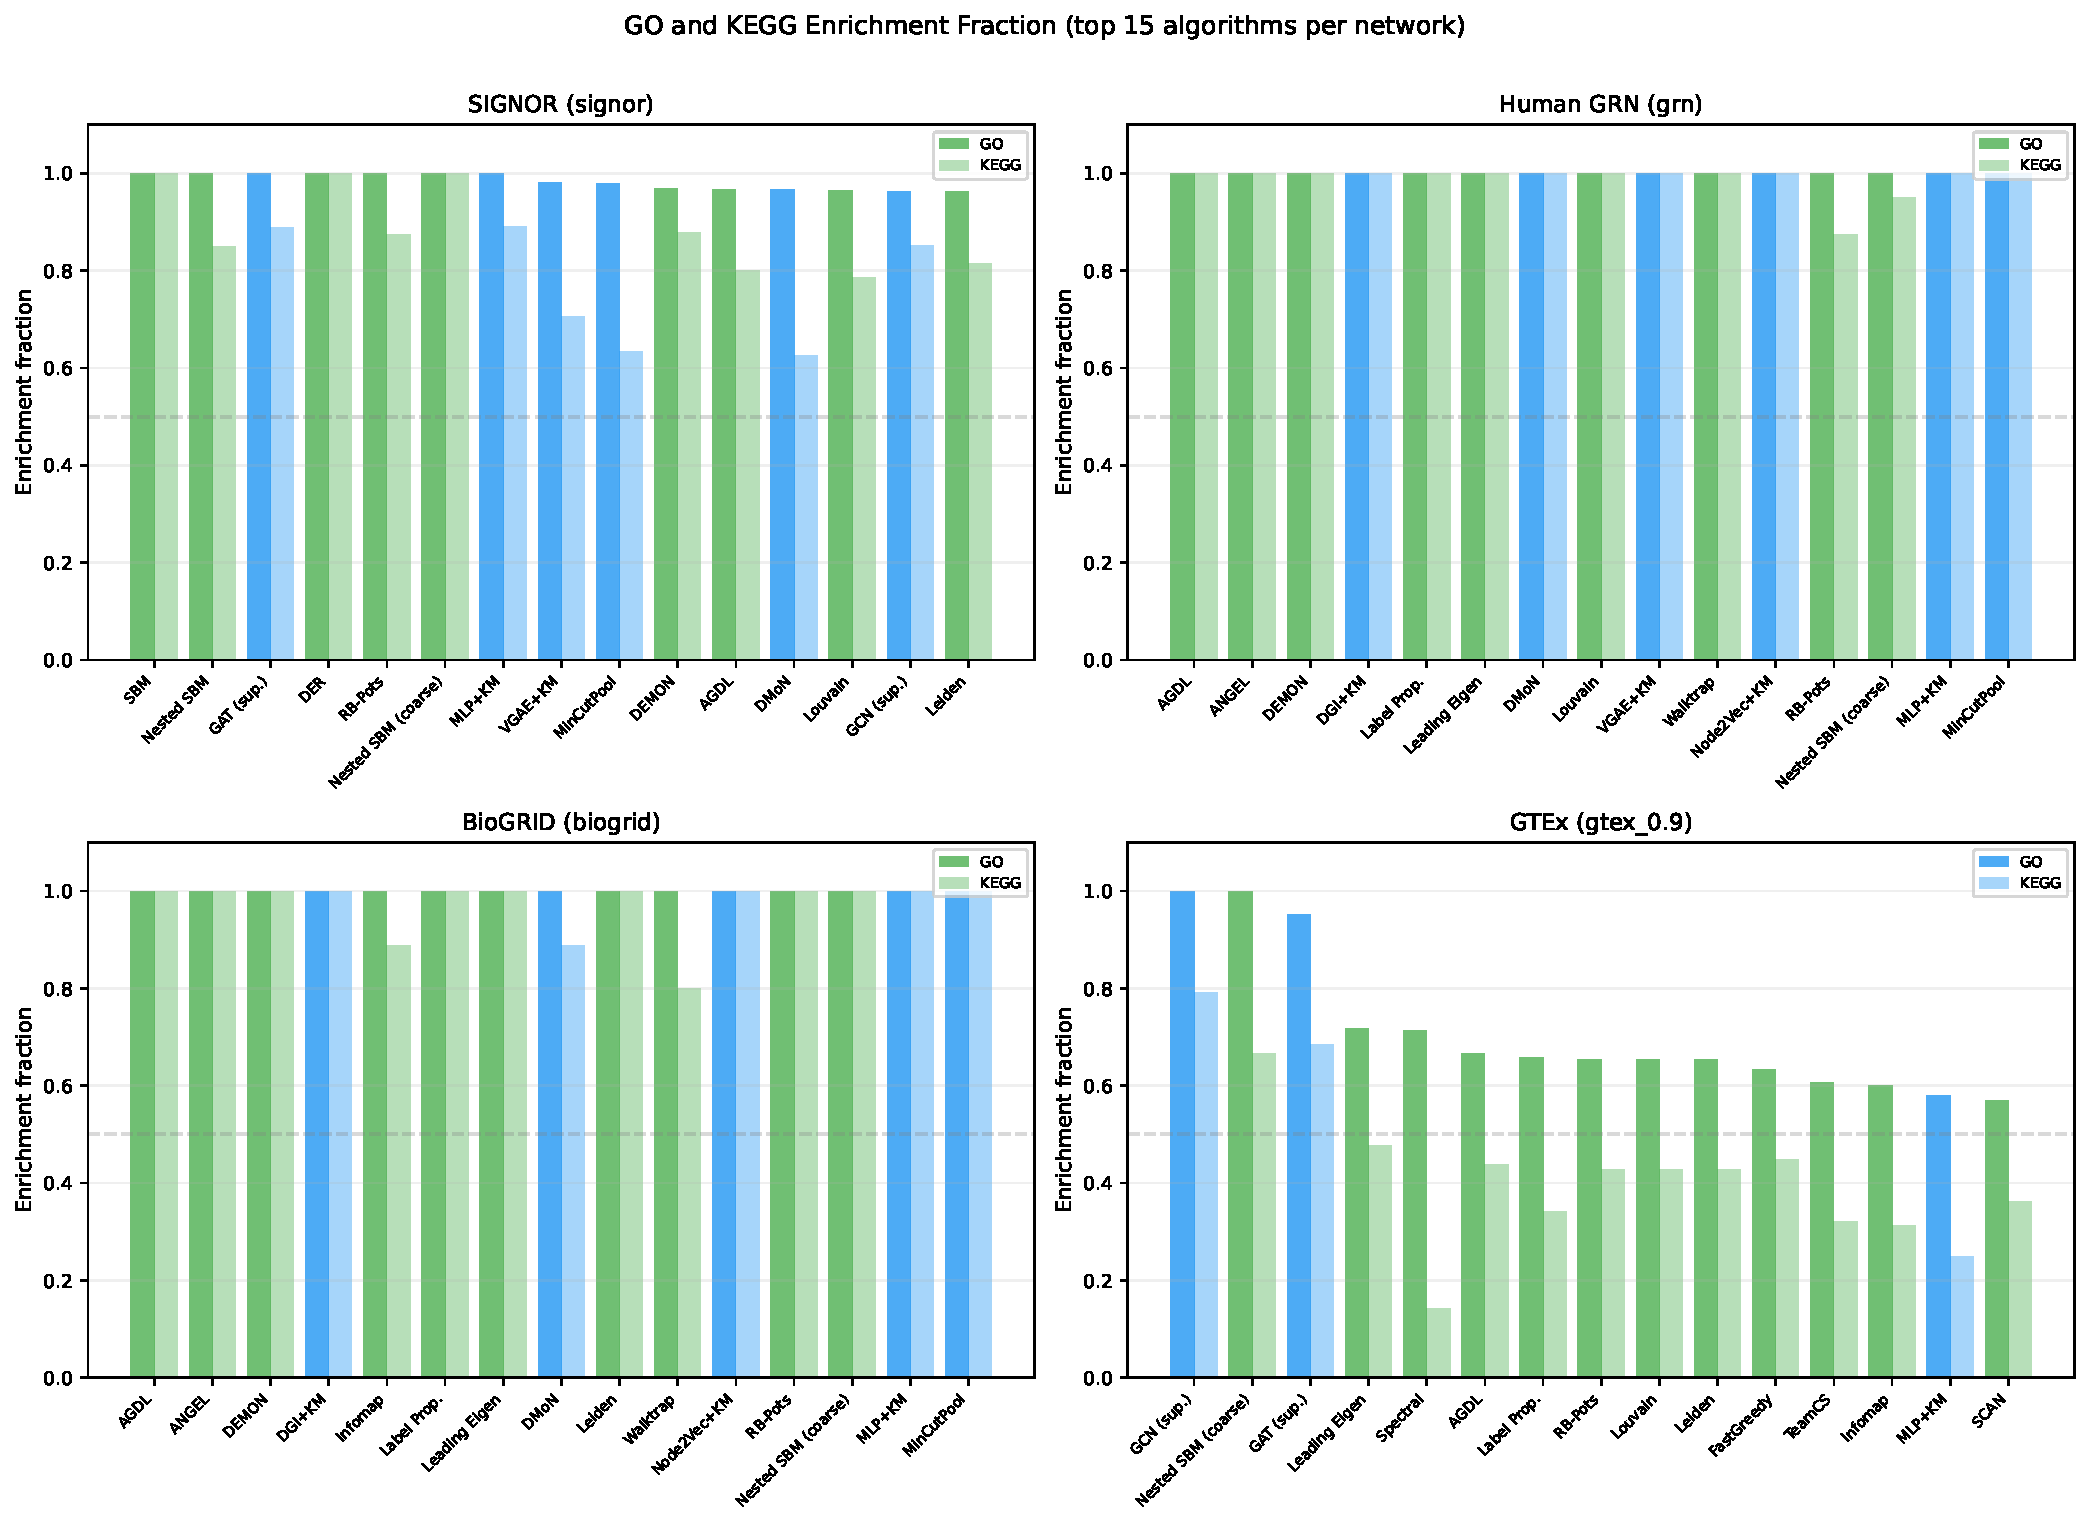
\includegraphics[width=\textwidth]{figures/fig_bio_enrichment.pdf}
\caption{GO and KEGG enrichment fractions (top~15 algorithms per network). Green bars: classical; blue bars: GNN. Solid bars: GO; translucent bars: KEGG. Communities with $\geq5$ nodes are tested (BH-adjusted $p<0.05$).}
\label{fig:bio_enrichment}
\end{figure}

Resolution dominates enrichment results (Figure~\ref{fig:bio_enrichment}).
This is not surprising (a community of 500 genes will almost certainly overlap some GO term), but the magnitude of the effect is striking.
On BioGRID, Leiden (K=8), Louvain (K=7), and RB-Pots (K=7) achieve 100\% enrichment for both GO and KEGG simply by producing a handful of large communities.
Meanwhile, CPM (K$>$1{,}000) manages only 35--53\% GO enrichment: many of its small communities lack the statistical power to reach significance, regardless of biological content.

After accounting for this resolution confound, do GNNs contribute additional value?
On three of four networks, yes: SIGNOR (mean GO enrichment 0.95 for GNNs vs 0.85 classical), GRN (1.00 vs 0.75), and BioGRID (1.00 vs 0.85).
However, GTEx reveals the opposite pattern.
There, unsupervised GNNs (DMoN, Node2Vec) fragment the dense co-expression graph into 300--400 small communities with poor enrichment ($\approx$0.30), while classical methods at moderate resolution achieve 0.65--0.72.
The pattern mirrors our Tier-2 finding precisely: GNNs improve performance when features carry biological signal that topology misses, but on dense graphs where topology alone is highly informative, they confer no advantage and may even degrade performance through over-fragmentation.

A quiet success: SBM and Nested SBM achieve perfect GO enrichment on SIGNOR and GRN by inferring a biologically natural resolution (K=13--56) without any user-specified parameters, an appealing property for exploratory biological analysis where the ``right'' number of modules is unknown.

\subsubsection{Sign Coherence (SIGNOR)}

Sign coherence on SIGNOR (the fraction of intra-community edges sharing a single regulatory sign) reveals an instructive tension.
The winners here are SCAN (0.88), MLP+KM (0.87), and Label Propagation (0.87): methods that carve out small, tightly-connected clusters where all edges tend to be activating or all inhibiting.
However, these are not the same algorithms that lead on pathway enrichment.
SBM and Nested SBM score perfect GO enrichment yet only mediocre sign coherence (0.66--0.69).
The reason is that these represent fundamentally distinct biological objectives.
Pathway membership groups genes by shared function regardless of regulatory direction; sign coherence rewards clusters where regulation flows uniformly.
A community detection method cannot optimize both simultaneously, and practitioners should select their metric based on their biological question.

\subsubsection{Perturbation Analysis (GRN)}

\begin{figure}[ht]
\centering
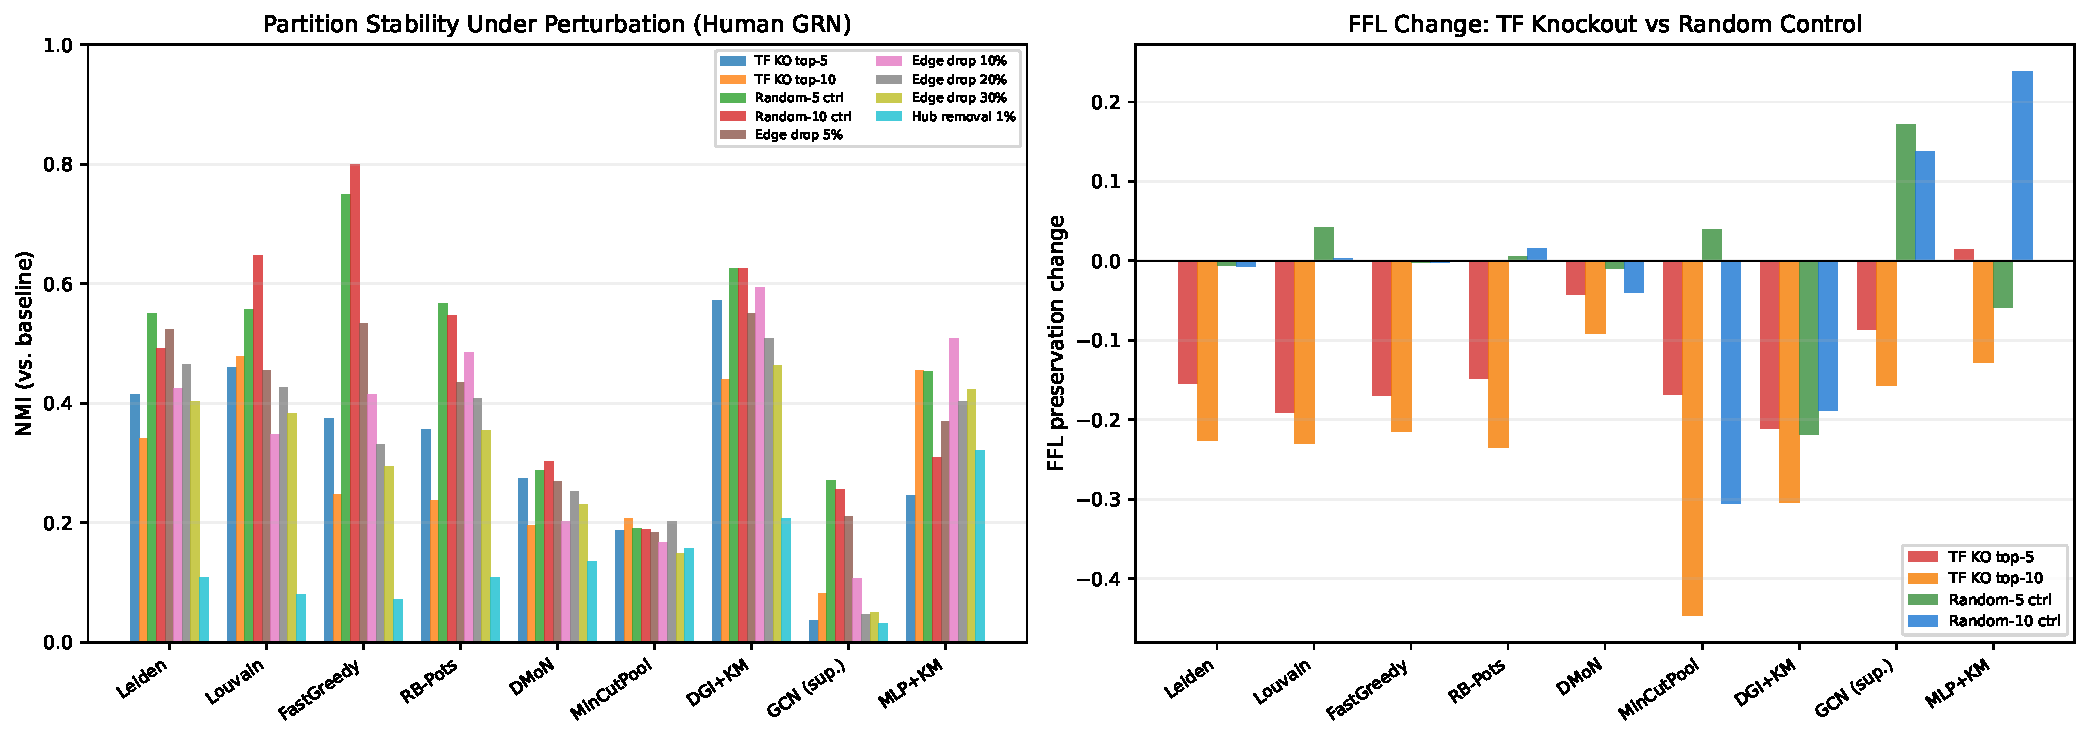
\includegraphics[width=\textwidth]{figures/fig_bio_perturbation.pdf}
\caption{Left: NMI between baseline and perturbed partitions across perturbation types on Human GRN. Right: FFL preservation change ($\Delta$FFL) for TF knockout vs random-gene controls.}
\label{fig:bio_perturbation}
\end{figure}

The perturbation analysis poses a pointed biological question: do the communities we detect reflect genuine regulatory organization, or are they arbitrary graph cuts that would appear equally disrupted under any perturbation?

We test this on the Human GRN (17{,}348 nodes, 264{,}393 edges; Figure~\ref{fig:bio_perturbation}) by comparing targeted perturbations (TF knockout, hub removal) against random controls (random gene removal).
The answer is unambiguous.
Removing just 5 transcription factors (by out-degree) drops partition NMI to 0.007--0.60, while removing 5 random genes yields NMI of 0.03--0.56.
For most algorithms, TF knockout is substantially more disruptive than random gene removal: FastGreedy shows the largest gap (NMI drops from 0.75 to 0.37 with top-5 knockout, a gap of 0.37 vs random control), and at top-10 the gap widens to 0.55.

Several algorithm-specific patterns emerge.
DGI is the most stable GNN overall (mean NMI = 0.51 across all perturbations), outperforming all classical methods; Node2Vec (NMI = 0.50) is comparably robust.
Their contrastive and random-walk objectives capture global structure that persists under local disruption.
In stark contrast, supervised GNNs (GAT: NMI = 0.05, GCN: NMI = 0.14) produce the most brittle partitions; their dependence on label-based optimization makes them fragile when the network structure changes.
Classical greedy methods (Leiden = 0.42, Louvain = 0.42) occupy the middle ground.

Under edge dropout, classical methods degrade more steeply (NMI: 0.48 at 5\% to 0.36 at 30\%) while GNNs degrade more slowly (0.34 to 0.31), suggesting that GNNs encode redundant representations that are less sensitive to individual edge loss.

\subsubsection{Feature Ablation on Biological Networks}

\begin{figure}[ht]
\centering
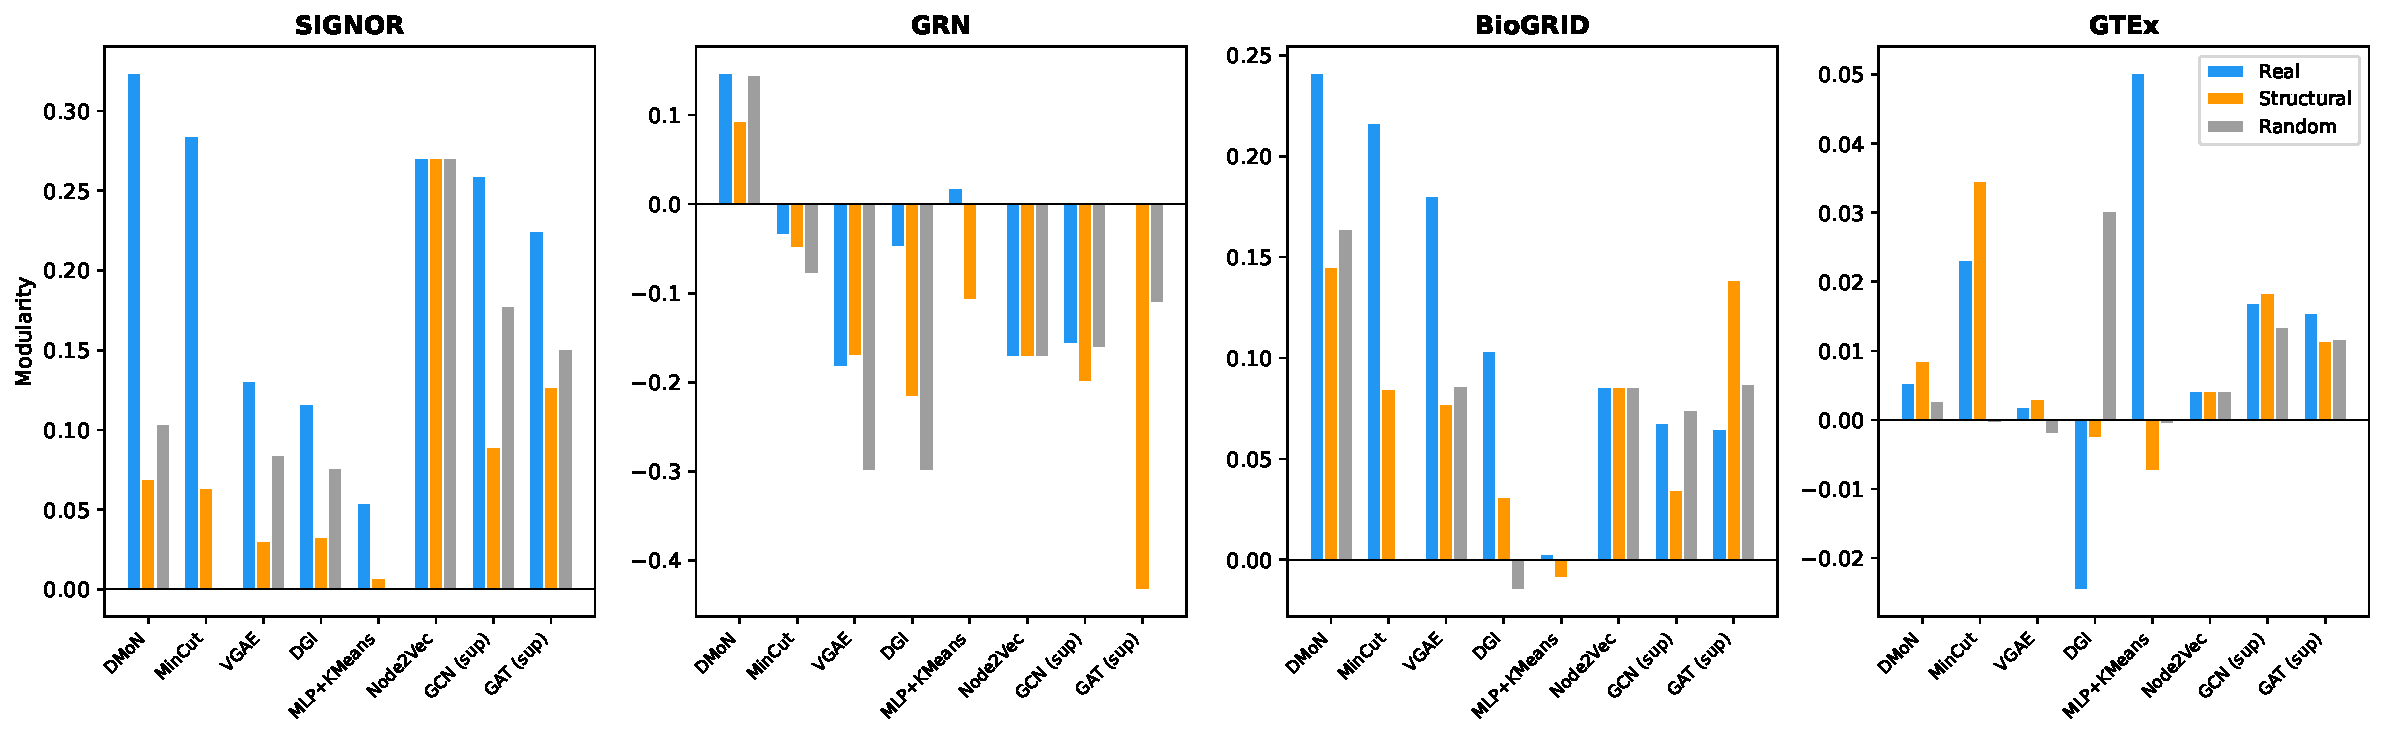
\includegraphics[width=\textwidth]{figures/bio_feature_ablation_modularity.pdf}
\caption{Biological feature ablation: mean modularity across 3 seeds for each GNN architecture under real biological features (expression PCA-128 or GO binary), structural features (degree + clustering coefficient + PageRank + spectral PE, 16-dim), and random Gaussian noise matching the real feature dimensionality.}
\label{fig:bio_feature_ablation}
\end{figure}

To directly test whether biological features (expression profiles, GO annotations) contribute signal beyond network topology on real molecular networks, we replicate the social-network ablation from Tier~2 on all four biological graphs.
Each of the 8 GNN architectures is trained with three feature settings: real biological features, 16-dimensional structural features (degree, clustering coefficient, PageRank, spectral positional encoding), and random Gaussian noise of matching dimensionality.

The results (Figure~\ref{fig:bio_feature_ablation}) confirm and extend the density-dependent principle we established on social networks.
On SIGNOR and BioGRID, which are relatively sparse networks where topology alone provides limited information, real biological features substantially outperform both structural and random alternatives.
Across all 8 GNN architectures, real features boost mean modularity by +93\% on SIGNOR and +100\% on BioGRID relative to random features; on GRN, the improvement is +56\%.
DMoN on SIGNOR achieves $Q = 0.324$ with real features vs $0.104$ with random (+212\%), confirming that GO-term annotations encode community structure that topology alone misses.

On GTEx, the densest network with $>$1.4M edges and 5{,}694 nodes, the feature advantage narrows to +56\%, and several GNNs perform comparably regardless of feature type.
This mirrors the Amazon Photo pattern from Tier~2 exactly.
Topology dominates: the dense co-expression graph already encodes most of the community signal in its edge weights, leaving little for node features to add.

Structural features occupy a consistent middle ground across all four networks.
They outperform random noise (validating that degree and clustering coefficient carry partial community information) but fall short of the biological features on sparse networks.
Node2Vec serves as an informative control: because it ignores node features entirely and learns from random walks, its performance is identical across all three feature settings.
This ordering (real $>$ structural $>$ random on sparse, all approximately equal on dense) generalizes the social-network finding to the biological domain and provides the first direct evidence that \emph{biological annotations earn their encoding cost specifically on the networks where they are most needed.}

\subsubsection{GNN Embedding Visualization}

\begin{figure}[ht]
\centering
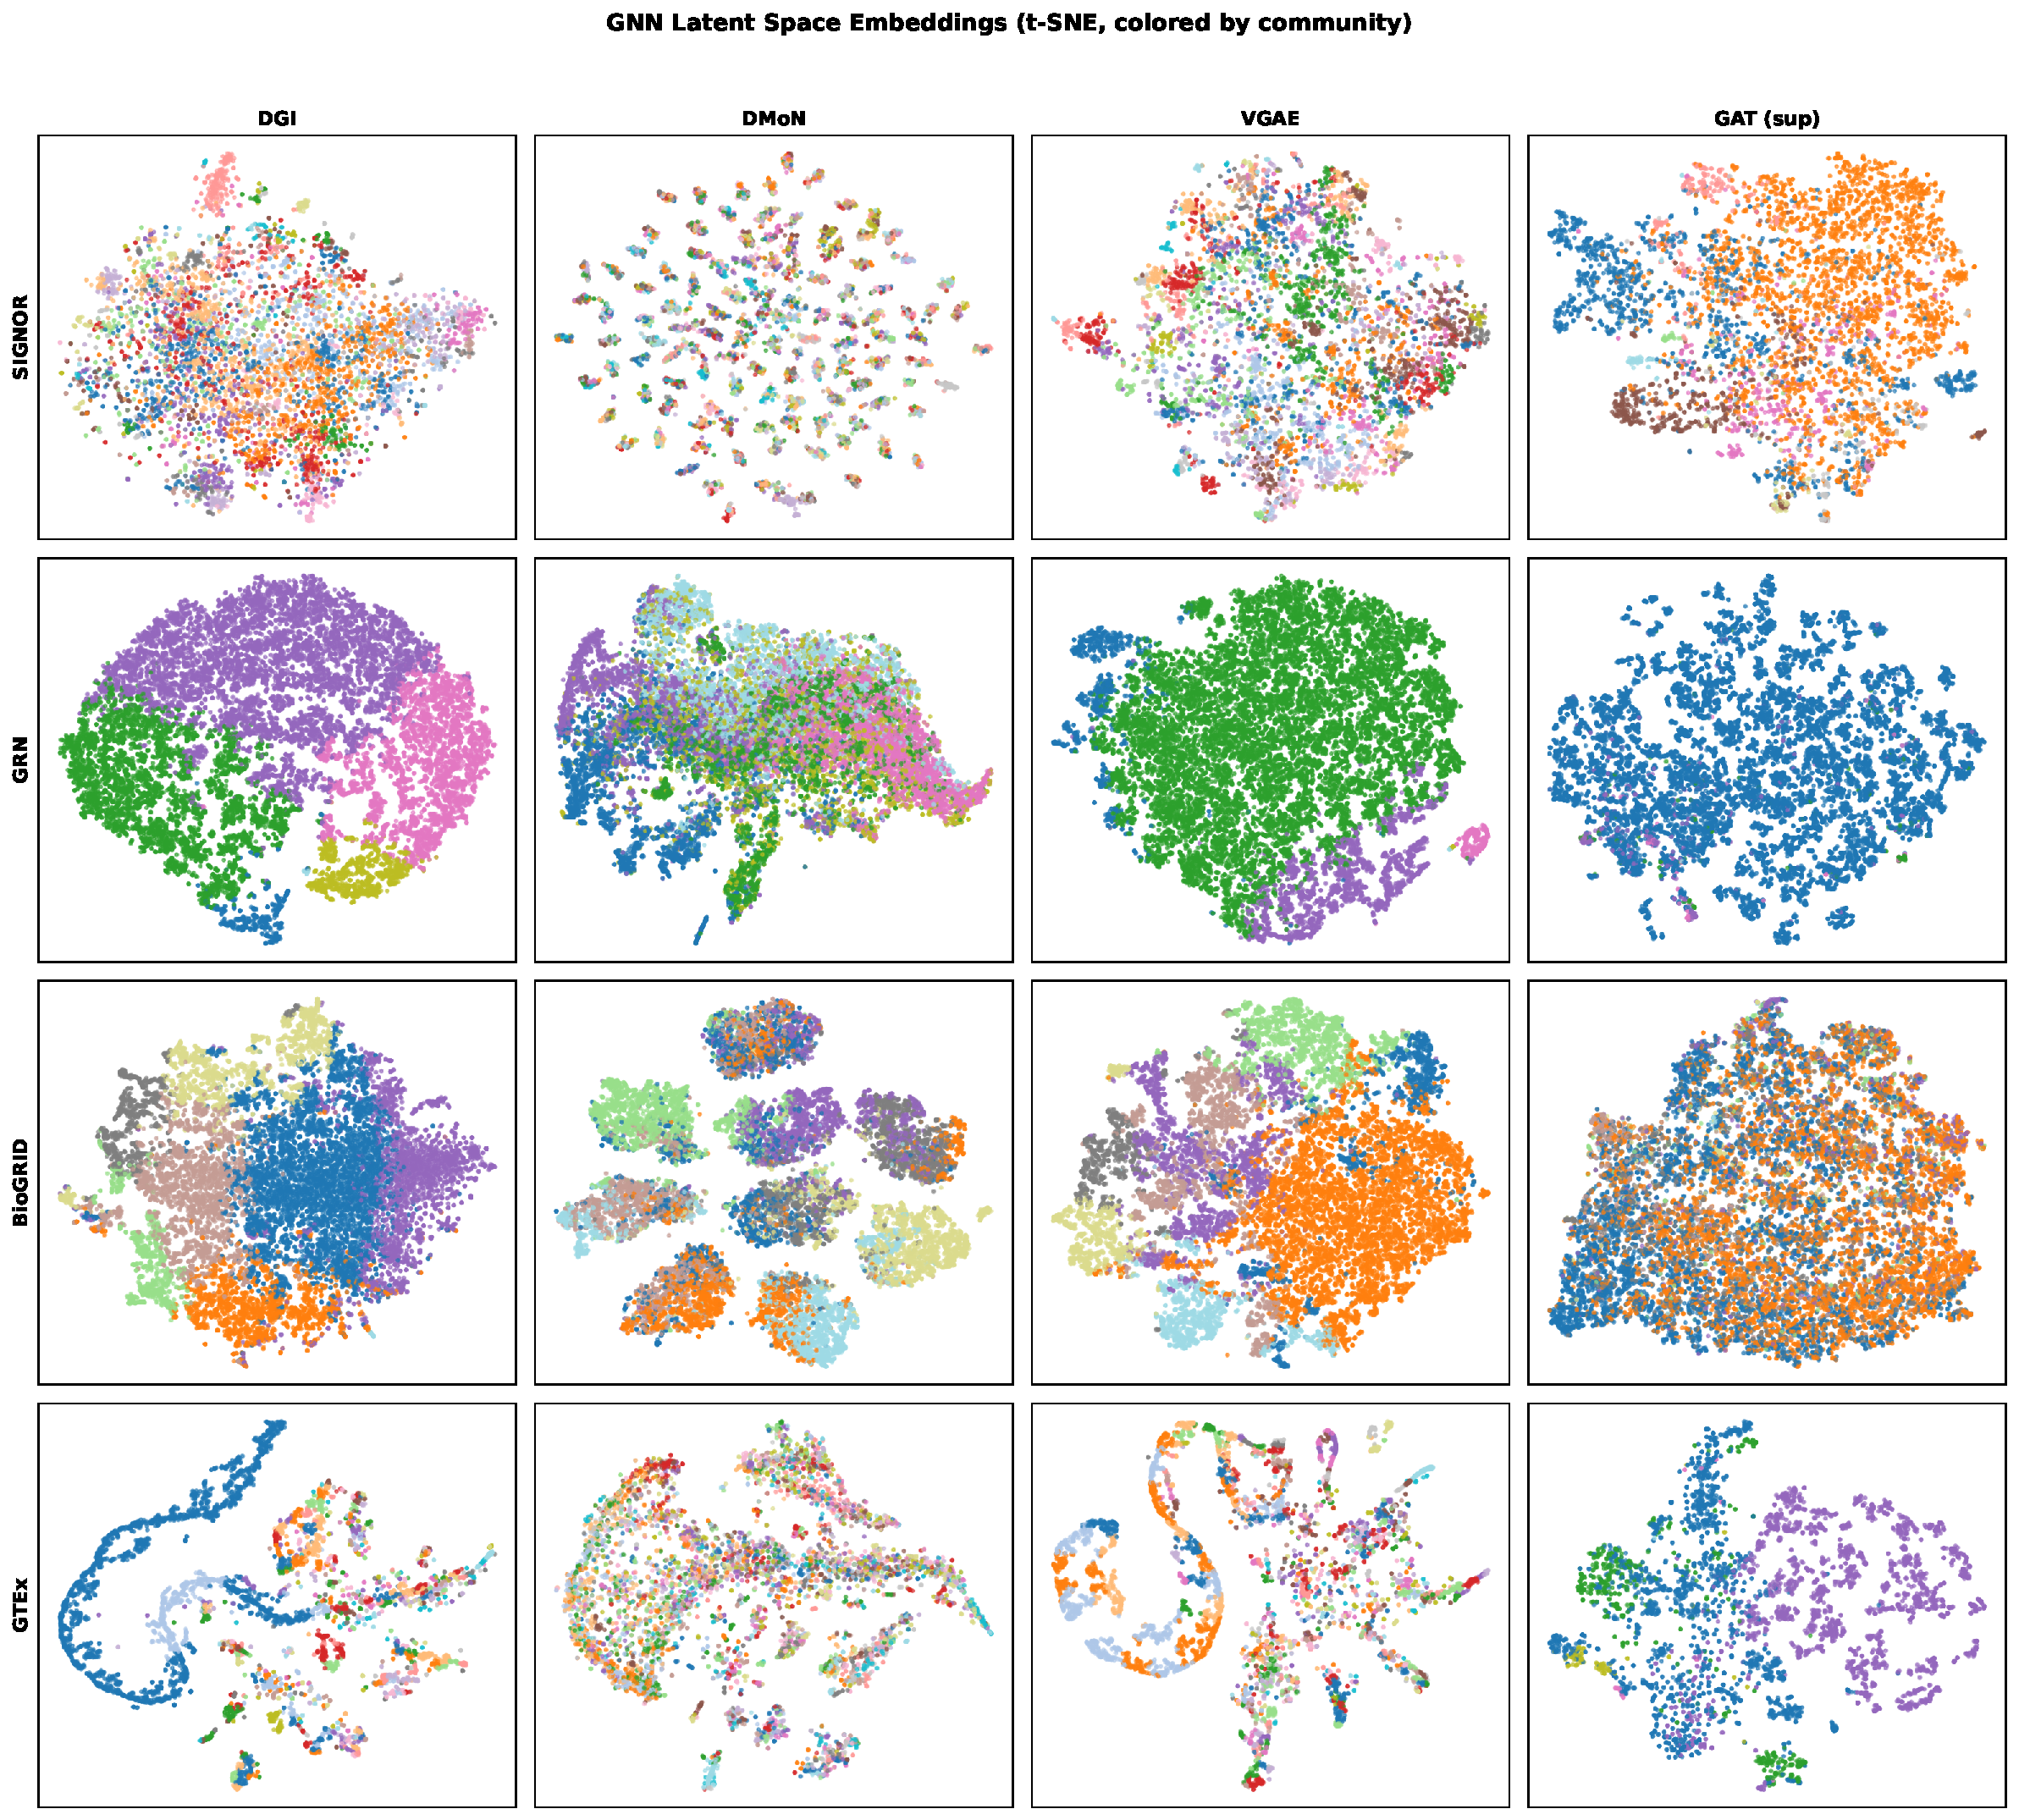
\includegraphics[width=\textwidth]{figures/bio_embedding_tsne_composite.pdf}
\caption{t-SNE projections of learned \textbf{node} embeddings from four GNN architectures on biological networks (rows: networks; columns: models). Each point represents a gene (node), positioned according to its 128-dimensional latent representation learned during training, and colored by its detected community assignment. DGI embeddings form well-separated clusters on SIGNOR and GRN, indicating that its contrastive objective learns discriminative per-gene representations. DMoN and VGAE produce more diffuse latent spaces on GTEx, consistent with the limited topological contrast in dense co-expression graphs.}
\label{fig:bio_embeddings}
\end{figure}

To visualize what different GNN architectures ``learn'' about biological network structure, we export latent embeddings from four representative models (DGI, DMoN, VGAE, GAT) and project them via t-SNE (Figure~\ref{fig:bio_embeddings}).

The visualization reveals striking architectural differences.
DGI, which maximizes mutual information between node and graph representations, produces the most clearly separated embedding clusters on SIGNOR and GRN, consistent with its strong perturbation robustness.
DMoN's modularity-based loss creates broader cluster boundaries, while VGAE's reconstruction objective produces embeddings where communities overlap substantially in latent space.
On GTEx, all architectures struggle to produce well-separated clusters, consistent with their poor enrichment performance: the dense graph provides insufficient topological contrast between communities for GNNs to exploit.

When colored by GO Slim biological category rather than detected community, DGI embeddings show partial separation by pathway function: genes involved in signaling, immune response, and cell cycle form distinct regions.
This provides visual evidence that the contrastive objective has learned biologically meaningful representations rather than arbitrary graph cuts.

\subsubsection{GAT Attention Weight Analysis}

\begin{figure}[ht]
\centering
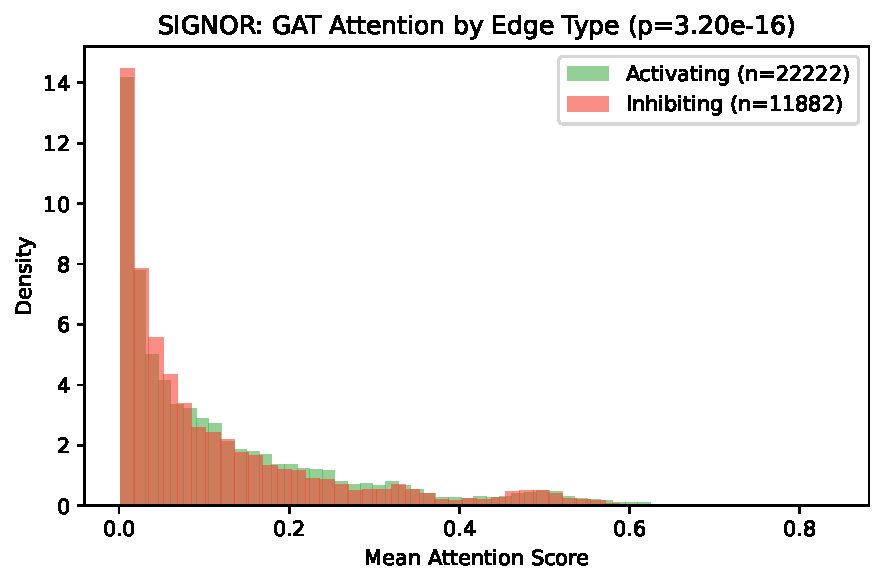
\includegraphics[width=0.7\textwidth]{figures/signor_attention_by_sign.pdf}
\caption{Distribution of GAT attention weights on SIGNOR edges, stratified by regulatory sign. Each edge receives a learned attention score during message passing; activating (positive-weight) edges receive significantly higher mean attention (0.123 vs 0.112, Mann-Whitney $p = 3.2 \times 10^{-16}$), indicating that the model attends preferentially to co-regulatory interactions that define within-community relationships.}
\label{fig:attention_signor}
\end{figure}

\begin{figure}[ht]
\centering
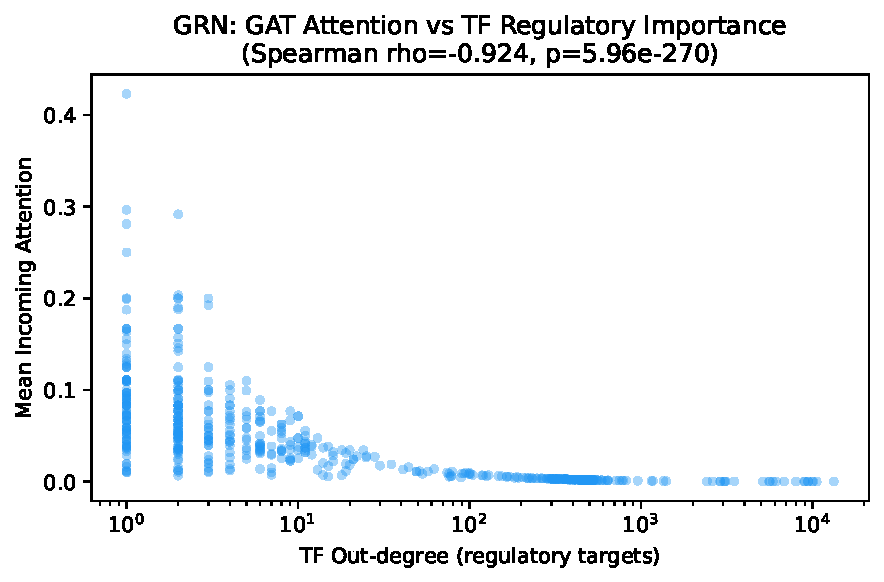
\includegraphics[width=0.6\textwidth]{figures/grn_attention_vs_outdegree.pdf}
\caption{Relationship between GAT per-node attention and transcription-factor (TF) out-degree on the human GRN. Each point represents one TF ($n = 642$); the $y$-axis shows the mean attention weight received by that TF's outgoing edges during message passing. The strong negative correlation (Spearman $\rho = -0.92$) demonstrates that GAT concentrates attention on specific, low-out-degree regulators rather than highly connected hub TFs, learning without explicit supervision that regulatory specificity carries more community-discriminative signal than regulatory breadth.}
\label{fig:attention_grn}
\end{figure}

The multi-head attention mechanism in GAT assigns learned importance weights to each edge.
We extract these weights after training and ask: does GAT attend preferentially to biologically meaningful edges?

On SIGNOR, we classify each edge as activating ($w > 0$) or inhibiting ($w < 0$) and compare attention score distributions (Figure~\ref{fig:attention_signor}).
Activating edges receive significantly higher mean attention (0.123) than inhibiting edges (0.112; Mann-Whitney $p = 3.2 \times 10^{-16}$, $n_{\text{act}} = 22{,}222$, $n_{\text{inh}} = 11{,}882$), indicating that GAT has learned to preferentially attend to positive regulatory interactions.
This is biologically plausible: activating edges often connect genes in shared pathways where co-regulation is the norm, while inhibiting edges connect antagonistic partners that belong to different functional modules.

On the GRN, we correlate per-node incoming attention with transcription-factor out-degree, a measure of regulatory influence (Figure~\ref{fig:attention_grn}).
Strikingly, attention shows a strong \emph{negative} correlation with out-degree (Spearman $\rho = -0.924$, $p = 5.96 \times 10^{-270}$, $n = 642$ TFs): GAT concentrates attention on \emph{specific} regulators (low out-degree) rather than master regulators (high out-degree).
This is biologically interpretable: hub TFs regulate hundreds of genes across multiple pathways non-specifically, so their edges carry less discriminative power for community membership.
Specific regulators that target only a few genes within a single module provide more informative edges for community detection.
This attention pattern was not explicitly trained into the model; it emerges from the semi-supervised objective of predicting GO Slim category, yet it recapitulates a biologically meaningful distinction between promiscuous and specific regulation.

These findings demonstrate that GNN attention mechanisms learn biologically interpretable structure, providing a form of model explainability for community detection that classical algorithms inherently lack.

\subsubsection{Disease Module Recovery (BioGRID)}

\begin{figure}[ht]
\centering
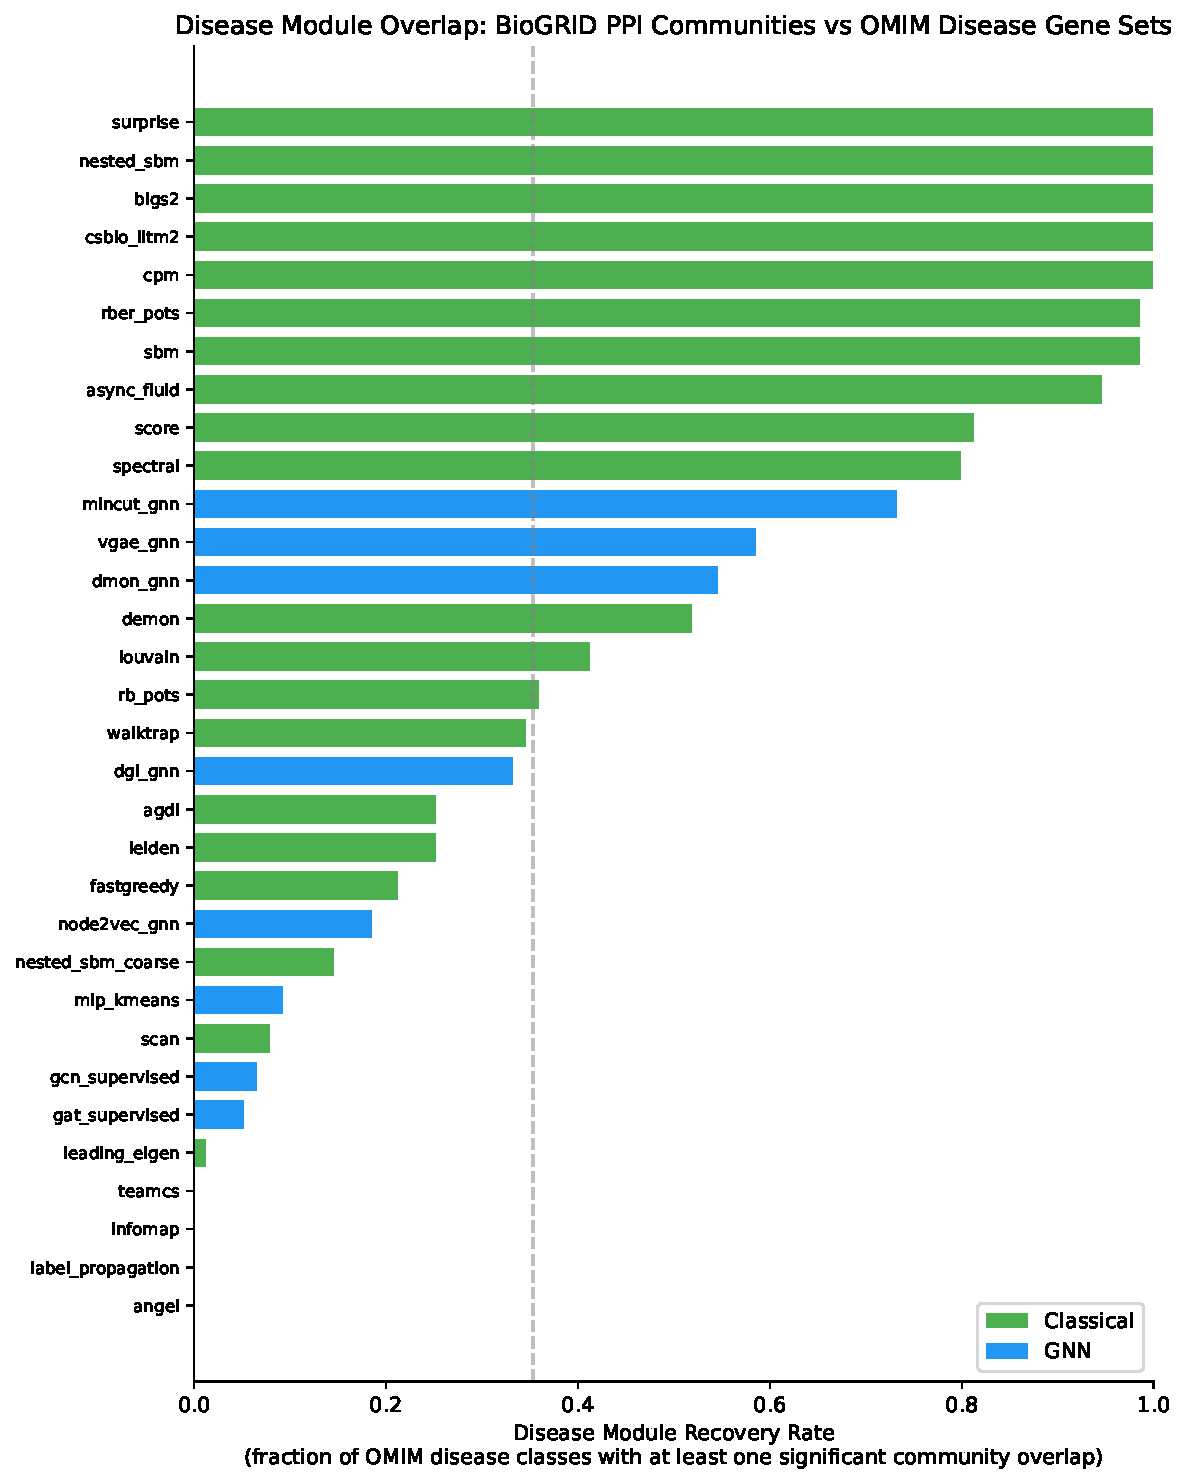
\includegraphics[width=\textwidth]{figures/fig_bio_disease_overlap.pdf}
\caption{Disease module recovery on BioGRID: fraction of 76 OMIM disease classes (each with $\geq$10 known disease genes in BioGRID) for which at least one detected community shows significant overlap (Fisher exact test, BH-corrected $p < 0.05$). Green: classical; blue: GNN.}
\label{fig:bio_disease_overlap}
\end{figure}

To test whether detected communities correspond to disease-relevant gene modules, we cross-referenced BioGRID PPI partitions against 76 OMIM disease gene sets (each with $\geq$10 genes present in BioGRID).
For each algorithm, we ask: what fraction of disease classes have at least one community with statistically significant gene overlap (Fisher exact test, BH correction at $p < 0.05$)?

The results (Figure~\ref{fig:bio_disease_overlap}) again highlight the resolution dependence we observed in enrichment analysis.
Methods producing many communities (CPM, Surprise, BigS2, CSBIO-IITM2, Nested SBM) recover $\geq$98\% of disease classes, because with hundreds of communities, at least one is likely to overlap any reasonably common disease gene set.
Methods producing very few communities (Infomap with $K=1$, Label Propagation with $K=1$) recover nothing.

Among GNNs, MinCutPool leads at 73\% recovery, followed by VGAE (59\%) and DMoN (55\%).
Semi-supervised GCN and GAT score poorly (5--7\%), consistent with their tendency to produce a small number of class-aligned communities that miss the combinatorial diversity of disease gene sets.
The practical conclusion: for disease module discovery on PPI networks, algorithms that naturally produce moderate-to-high resolution partitions (50--200 communities) outperform both extremes.


% ============================================================================
\section{Discussion}
\label{sec:discussion}

\subsection{When Do GNNs Actually Help?}

The central question motivating this work deserves a nuanced answer.
Our three tiers trace a clear conditional:

\emph{GNNs help when (1) the network is sparse enough that topology alone leaves ambiguity, AND (2) node features carry genuine information about community membership.}

On LFR graphs, where communities are defined entirely by edge density, GNNs contribute nothing and incur a substantial computational overhead for consuming uninformative structural features.
On social networks, features improve performance in direct proportion to their informativeness: bag-of-words on sparse citation graphs yield large AMI gains, while random features on dense Amazon Photo barely diminish semi-supervised methods.
On biological networks, the prediction holds: GNNs outperform classical methods on SIGNOR, GRN, and BioGRID (networks where GO-term or expression features encode biological function that topology cannot fully capture) but underperform on GTEx, where the dense co-expression graph already encodes most of the relevant structure in its edge weights.

This suggests a practical decision rule for biologists: if your network has fewer than ${\sim}10^5$ edges per thousand nodes and you have meaningful per-gene annotations (expression profiles, GO terms, protein domains), a GNN is likely worth the setup cost.
If your network is dense and you lack informative node features, Leiden will finish in seconds and give comparable or better results.

\subsection{Why Does Resolution Confound Biological Evaluation?}

The strong dependence of enrichment scores on community size deserves more discussion than it typically receives.
An algorithm that produces 7 communities on a 15{,}000-gene PPI network will almost certainly achieve 100\% GO enrichment because each community spans thousands of genes and overlaps dozens of pathways.
An algorithm producing 1{,}000 communities gives a finer-grained partition that may better reflect individual pathway boundaries, but many communities will be too small to reach statistical significance in a hypergeometric test.

This is not a flaw in either algorithm; it reflects a genuine biological ambiguity about what ``community'' means.
Is a module the entire set of genes involved in immune signaling, or a specific subcomplex within that pathway?
Our results show that resolution choice implicitly answers this question, and different downstream applications demand different answers.
Drug target discovery may benefit from fine-grained communities (each corresponding to a specific mechanism); pathway-level annotation benefits from coarse partitions that maximize enrichment power.
The disease module analysis (Figure~\ref{fig:bio_disease_overlap}) makes this concrete: algorithms with 50--200 communities recover the most OMIM disease classes, while both extremes (1 community or $>$1{,}000) perform poorly for different reasons.
We recommend that biological benchmarks always report enrichment alongside community count, and that practitioners explicitly state their desired resolution before choosing an algorithm.

\subsection{The Tension Between Pathway Enrichment and Regulatory Coherence}

The sign coherence results on SIGNOR reveal something that enrichment-only evaluations miss entirely.
SBM produces communities that are maximally enriched for GO terms but internally incoherent in regulatory sign, mixing activating and inhibiting edges freely.
SCAN produces the opposite: highly sign-coherent communities that are less functionally enriched.

We interpret this as reflecting two distinct levels of biological organization.
Functional modules (what GO captures) group genes by shared downstream effect regardless of how they regulate one another.
Regulatory modules (what sign coherence captures) group genes by shared regulatory logic: uniformly activated or uniformly repressed.
These represent fundamentally different organizational principles, and no single algorithm can optimize both simultaneously.
For signaling network analysis, we recommend applying both a coarse method (SBM or Leiden for pathway annotation) and a local method (SCAN or Label Propagation for regulatory circuit identification), then comparing the resulting partitions.

\subsection{What the Perturbation Analysis Means for Drug Target Prioritization}

The disproportionate effect of TF knockout on community structure has implications beyond benchmarking.
If removing a single transcription factor reshuffles communities while removing a random gene does not, then community membership is encoding regulatory dependency.
Genes that appear in the same community as a high-out-degree TF are, in a meaningful sense, ``downstream'' of that regulator.

This connects to an active area in drug discovery: predicting which targets, when inhibited, will maximally disrupt a disease-relevant module.
Our perturbation analysis suggests that community detection could serve as a computationally inexpensive proxy for influence estimation, more tractable than full network propagation and more interpretable than learned attention weights.
The 5\%-hub catastrophe threshold also has practical implications: it defines the point beyond which a disease has damaged so many network hubs that modular structure is no longer recoverable, potentially corresponding to a therapeutic ``point of no return.''

\subsection{What GAT Attention Reveals About Network Biology}

The attention weight analysis provides a concrete demonstration of what AI-based community detection can offer beyond partitions: biological interpretation at the edge level.
Classical algorithms produce communities but provide no insight into \emph{why} particular nodes were grouped together.
GAT's attention mechanism, by contrast, quantifies the contribution of each edge to the final clustering, creating a per-edge importance map that is both learned and interpretable.

Three findings from our attention analysis have biological implications.
First, the preferential attention to activating edges on SIGNOR ($p = 3.2 \times 10^{-16}$) suggests that pathway-level co-regulation is a stronger clustering signal than antagonistic regulation, consistent with the biological intuition that co-activated genes form modules.
Second, the strong negative correlation between attention and TF out-degree on the GRN ($\rho = -0.92$) reveals that GAT concentrates on \emph{specific} regulators rather than master regulators.
This is biologically interpretable: hub TFs regulate many pathways simultaneously and thus carry low discriminative power for community membership, while specific TFs targeting few genes within one module provide the sharpest community-defining edges.
The model has learned, without explicit instruction, that regulatory specificity matters more than regulatory breadth for partitioning.
Third, the attention entropy varies across networks: SIGNOR and GRN show non-uniform attention (the model is being selective), while GTEx attention is nearly uniform (the dense graph provides no strong edge-level signal), consistent with GTEx being the one network where GNNs fail to outperform classical methods.

These attention-derived insights complement traditional pathway analysis and suggest a genuinely new application of GNN-based community detection: not just producing partitions, but identifying the edges and nodes that drive community formation.
For regulatory networks, attention-weighted edges could highlight the most functionally important regulatory relationships, a form of data-driven edge prioritization that requires no prior pathway knowledge.

\subsection{Practitioner Guidelines}

For researchers approaching a new biological network without strong prior assumptions:

\begin{enumerate}[leftmargin=*]
  \item \textbf{Start with Leiden or Louvain.} They are fast, robust, and competitive across all network types. Use them as a baseline even if you plan to try GNNs.
  \item \textbf{Try a GNN only if you have informative node features.} Gene expression profiles, GO annotations, or protein domain features all qualify. Degree-based structural features do not.
  \item \textbf{Use Nested SBM for exploratory hierarchical analysis.} It automatically selects resolution and resists the modularity resolution limit.
  \item \textbf{Do not trust modularity alone.} Supplement with GO/KEGG enrichment, motif preservation, or domain-appropriate coherence metrics.
  \item \textbf{At $N > 10{,}000$}, stick to near-linear methods. Quadratic-time algorithms (Spectral, Spinglass) become impractical and offer no accuracy advantage on large biological networks.
  \item \textbf{Report community count alongside performance.} Without this, enrichment comparisons are uninterpretable.
\end{enumerate}

\subsection{Limitations}

Several limitations temper our conclusions.
First, GNN hyperparameters were not exhaustively tuned per dataset; aggressive architecture search could close some of the gap with classical methods, though we doubt it would reverse the overall pattern on featureless graphs.
Second, our biological enrichment relies on g:Profiler's current GO annotation database, which inherently favors communities whose size matches the size distribution of GO terms, a bias shared by all enrichment-based evaluations in the literature.
Third, the LFR generator does not produce attributed communities, so Tier~1 cannot test GNNs under their intended use case; this is by design (we want to establish what happens \emph{without} features) but limits generalizability.
Fourth, the attention analysis uses a semi-supervised GAT trained on GO Slim labels; biases in GO annotation coverage could influence which edges receive high attention.
Finally, we evaluate each algorithm independently, whereas ensemble approaches combining classical and GNN partitions may outperform any single method.


% ============================================================================
\section{Conclusion}
\label{sec:conclusion}

Four findings stand out from this benchmark, and together they tell a story about when and how AI adds value to biological network analysis.

First, GNNs are not universally superior to classical methods; they are \emph{conditionally} superior.
The condition is precise: informative node features on a network sparse enough that topology leaves genuine ambiguity about community boundaries.
When that condition holds (SIGNOR, GRN, BioGRID, sparse citation graphs), GNNs justify their computational overhead.
When it does not (LFR, GTEx), they are slower and no more accurate than Leiden.
We confirmed this principle directly on biological networks through feature ablation: GO annotations boost performance by 56--100\% on sparse regulatory networks but add negligible signal on dense co-expression graphs.

Second, and perhaps most significant for the AI-in-biology community, GNNs learn biologically interpretable structure that classical methods fundamentally cannot provide.
GAT attention weights preferentially attend to activating edges ($p = 3.2 \times 10^{-16}$) and concentrate on specific rather than promiscuous regulators ($\rho = -0.92$); embedding visualizations reveal pathway-aligned latent clusters; and these patterns emerge from generic semi-supervised objectives without explicit pathway supervision.
This interpretability enables genuinely new applications: attention-weighted edge prioritization for pathway discovery and embedding-based functional annotation of uncharacterized genes.

Third, biological networks demand biological metrics.
Modularity scores convey little about whether a detected partition corresponds to genuine pathways.
GO enrichment, FFL preservation, and sign coherence each capture a different axis of biological validity, and they do not always agree.
We observed that an algorithm can excel on one metric while performing poorly on another.
Single-metric evaluations are inadequate for biological community detection.

Fourth, community structure in regulatory networks is not an abstraction but reflects real transcriptional organization.
Removing five TFs reshuffles partitions far more than removing five random genes (NMI gap up to 0.55 for FastGreedy at top-10 knockout).
DGI emerges as the most perturbation-robust method (NMI = 0.51), while supervised GNNs (GAT, GCN) produce partitions that collapse under even mild perturbation (NMI $<$ 0.14).
This finding suggests that community detection, combined with targeted perturbation, could serve as a cheap screening tool for identifying regulatory bottlenecks and candidate drug targets.

Looking ahead, we believe the most promising direction lies not in better algorithms per se, but in deeper integration of biological knowledge into the detection process.
GNNs are the natural vehicle for this integration because they can consume arbitrary node or edge features as input, but realizing this potential requires features that genuinely encode biological function rather than trivially recapitulating topology.
The gap between GNN performance on well-annotated networks (SIGNOR, BioGRID) and poorly-annotated ones (GTEx with only PCA-compressed expression) makes this point quantitatively.
As biological databases grow richer, we expect the GNN advantage to grow with them.

All 38 algorithms are released as ClusterNet, a unified Python package with reproducible pipelines for all three tiers.
We hope ClusterNet will serve both as a practical tool for biologists choosing a community detection method and as a testbed for the AI community developing the next generation of graph learning algorithms for biology.


% ============================================================================
\section*{Data and Code Availability}

LFR networks are generated with the standard benchmark code~\citep{andrea_lancichinetti_125b2a5e}; social datasets auto-download via PyTorch Geometric~\citep{fey_pyg_2019}; biological networks derive from GTEx~\citep{gtex_2020}, BioGRID~\citep{biogrid_2023}, SIGNOR~\citep{signor_2020}, and the Gene Ontology Consortium~\citep{gene_ontology_2021}.
Code, data pipelines, and all analysis scripts are available as the ClusterNet package at \url{https://github.com/RamanLab/ClusterNet}.
Supplementary Tables~S1--S9 contain full numerical results for all tiers (S8: disease module overlap; S9: biological feature ablation); SHA-256 checksums and automated validation scripts (\texttt{validate\_lfr\_manuscript.py}, \texttt{validate\_social\_manuscript.py}, \texttt{validate\_biological\_manuscript.py}) ensure reproducibility.

\section*{Acknowledgments}

Computational experiments were performed on a single NVIDIA RTX 5090 GPU instance provisioned through Vast.ai.
The authors acknowledge the support of the PG Senapathy Center for Computing Resources at IIT Madras.

% ============================================================================
\bibliography{references}

\end{document}
